\documentclass[twoside]{book}

% Packages required by doxygen
\usepackage{fixltx2e}
\usepackage{calc}
\usepackage{doxygen}
\usepackage[export]{adjustbox} % also loads graphicx
\usepackage{graphicx}
\usepackage[utf8]{inputenc}
\usepackage{makeidx}
\usepackage{multicol}
\usepackage{multirow}
\PassOptionsToPackage{warn}{textcomp}
\usepackage{textcomp}
\usepackage[nointegrals]{wasysym}
\usepackage[table]{xcolor}

% Font selection
\usepackage[T1]{fontenc}
\usepackage[scaled=.90]{helvet}
\usepackage{courier}
\usepackage{amssymb}
\usepackage{sectsty}
\renewcommand{\familydefault}{\sfdefault}
\allsectionsfont{%
  \fontseries{bc}\selectfont%
  \color{darkgray}%
}
\renewcommand{\DoxyLabelFont}{%
  \fontseries{bc}\selectfont%
  \color{darkgray}%
}
\newcommand{\+}{\discretionary{\mbox{\scriptsize$\hookleftarrow$}}{}{}}

% Page & text layout
\usepackage{geometry}
\geometry{%
  a4paper,%
  top=2.5cm,%
  bottom=2.5cm,%
  left=2.5cm,%
  right=2.5cm%
}
\tolerance=750
\hfuzz=15pt
\hbadness=750
\setlength{\emergencystretch}{15pt}
\setlength{\parindent}{0cm}
\setlength{\parskip}{3ex plus 2ex minus 2ex}
\makeatletter
\renewcommand{\paragraph}{%
  \@startsection{paragraph}{4}{0ex}{-1.0ex}{1.0ex}{%
    \normalfont\normalsize\bfseries\SS@parafont%
  }%
}
\renewcommand{\subparagraph}{%
  \@startsection{subparagraph}{5}{0ex}{-1.0ex}{1.0ex}{%
    \normalfont\normalsize\bfseries\SS@subparafont%
  }%
}
\makeatother

% Headers & footers
\usepackage{fancyhdr}
\pagestyle{fancyplain}
\fancyhead[LE]{\fancyplain{}{\bfseries\thepage}}
\fancyhead[CE]{\fancyplain{}{}}
\fancyhead[RE]{\fancyplain{}{\bfseries\leftmark}}
\fancyhead[LO]{\fancyplain{}{\bfseries\rightmark}}
\fancyhead[CO]{\fancyplain{}{}}
\fancyhead[RO]{\fancyplain{}{\bfseries\thepage}}
\fancyfoot[LE]{\fancyplain{}{}}
\fancyfoot[CE]{\fancyplain{}{}}
\fancyfoot[RE]{\fancyplain{}{\bfseries\scriptsize Generated by Doxygen }}
\fancyfoot[LO]{\fancyplain{}{\bfseries\scriptsize Generated by Doxygen }}
\fancyfoot[CO]{\fancyplain{}{}}
\fancyfoot[RO]{\fancyplain{}{}}
\renewcommand{\footrulewidth}{0.4pt}
\renewcommand{\chaptermark}[1]{%
  \markboth{#1}{}%
}
\renewcommand{\sectionmark}[1]{%
  \markright{\thesection\ #1}%
}

% Indices & bibliography
\usepackage{natbib}
\usepackage[titles]{tocloft}
\setcounter{tocdepth}{3}
\setcounter{secnumdepth}{5}
\makeindex

% Hyperlinks (required, but should be loaded last)
\usepackage{ifpdf}
\ifpdf
  \usepackage[pdftex,pagebackref=true]{hyperref}
\else
  \usepackage[ps2pdf,pagebackref=true]{hyperref}
\fi
\hypersetup{%
  colorlinks=true,%
  linkcolor=blue,%
  citecolor=blue,%
  unicode%
}

% Custom commands
\newcommand{\clearemptydoublepage}{%
  \newpage{\pagestyle{empty}\cleardoublepage}%
}

\usepackage{caption}
\captionsetup{labelsep=space,justification=centering,font={bf},singlelinecheck=off,skip=4pt,position=top}

%===== C O N T E N T S =====

\begin{document}

% Titlepage & ToC
\hypersetup{pageanchor=false,
             bookmarksnumbered=true,
             pdfencoding=unicode
            }
\pagenumbering{alph}
\begin{titlepage}
\vspace*{7cm}
\begin{center}%
{\Large M\+C\+Network }\\
\vspace*{1cm}
{\large Generated by Doxygen 1.8.13}\\
\end{center}
\end{titlepage}
\clearemptydoublepage
\pagenumbering{roman}
\tableofcontents
\clearemptydoublepage
\pagenumbering{arabic}
\hypersetup{pageanchor=true}

%--- Begin generated contents ---
\chapter{M\+C\+Network}
\label{index}\hypertarget{index}{}\hypertarget{index_install_sec}{}\section{Installation}\label{index_install_sec}
\hypertarget{index_step1}{}\subsection{Step 1\+: Dependencies}\label{index_step1}
mfem (serial version)\+: \href{https://mfem.org/building/}{\tt https\+://mfem.\+org/building/} ~\newline
 boost ~\newline
\hypertarget{index_step2}{}\subsection{Step 2\+: Install}\label{index_step2}
git clone \href{https://github.com/MarlonBecker/MCNetwork}{\tt https\+://github.\+com/\+Marlon\+Becker/\+M\+C\+Network} ~\newline
 mkdir build ~\newline
 cd build ~\newline
 cmake .. ~\newline
 make ~\newline
\hypertarget{index_step3}{}\subsection{Step 3\+: Run Example}\label{index_step3}
cd data ~\newline
 ../build/\+M\+Cnetwork --mnd --opt\+MC --r\+SV ~\newline
 
\chapter{Hierarchical Index}
\section{Class Hierarchy}
This inheritance list is sorted roughly, but not completely, alphabetically\+:\begin{DoxyCompactList}
\item \contentsline{section}{Data\+File}{\pageref{classDataFile}}{}
\item \contentsline{section}{Electrode\+Parameters}{\pageref{structElectrodeParameters}}{}
\item \contentsline{section}{Finite\+Elemente\+Base}{\pageref{classFiniteElementeBase}}{}
\begin{DoxyCompactList}
\item \contentsline{section}{Finite\+Elemente\+Circle}{\pageref{classFiniteElementeCircle}}{}
\item \contentsline{section}{Finite\+Elemente\+Rect}{\pageref{classFiniteElementeRect}}{}
\end{DoxyCompactList}
\item \contentsline{section}{Job}{\pageref{classJob}}{}
\item \contentsline{section}{Job\+Manager}{\pageref{classJobManager}}{}
\item \contentsline{section}{my\+Debugger}{\pageref{classmyDebugger}}{}
\item \contentsline{section}{Optimizer}{\pageref{classOptimizer}}{}
\item \contentsline{section}{Parameter\+Storage}{\pageref{classParameterStorage}}{}
\item \contentsline{section}{System}{\pageref{classSystem}}{}
\end{DoxyCompactList}

\chapter{Data Structure Index}
\section{Data Structures}
Here are the data structures with brief descriptions\+:\begin{DoxyCompactList}
\item\contentsline{section}{\hyperlink{classDataFile}{Data\+File} }{\pageref{classDataFile}}{}
\item\contentsline{section}{\hyperlink{structElectrodeParameters}{Electrode\+Parameters} }{\pageref{structElectrodeParameters}}{}
\item\contentsline{section}{\hyperlink{classFiniteElementeBase}{Finite\+Elemente\+Base} }{\pageref{classFiniteElementeBase}}{}
\item\contentsline{section}{\hyperlink{classFiniteElementeCircle}{Finite\+Elemente\+Circle} }{\pageref{classFiniteElementeCircle}}{}
\item\contentsline{section}{\hyperlink{classFiniteElementeRect}{Finite\+Elemente\+Rect} }{\pageref{classFiniteElementeRect}}{}
\item\contentsline{section}{\hyperlink{classJob}{Job} }{\pageref{classJob}}{}
\item\contentsline{section}{\hyperlink{classJobManager}{Job\+Manager} }{\pageref{classJobManager}}{}
\item\contentsline{section}{\hyperlink{classmyDebugger}{my\+Debugger} }{\pageref{classmyDebugger}}{}
\item\contentsline{section}{\hyperlink{classOptimizer}{Optimizer} }{\pageref{classOptimizer}}{}
\item\contentsline{section}{\hyperlink{classParameterStorage}{Parameter\+Storage} }{\pageref{classParameterStorage}}{}
\item\contentsline{section}{\hyperlink{classSystem}{System} }{\pageref{classSystem}}{}
\end{DoxyCompactList}

\chapter{Data Structure Documentation}
\hypertarget{classDataFile}{}\section{Data\+File Class Reference}
\label{classDataFile}\index{Data\+File@{Data\+File}}


{\ttfamily \#include $<$datafile.\+h$>$}

\subsection*{Public Member Functions}
\begin{DoxyCompactItemize}
\item 
\hyperlink{classDataFile_a506afaa3e498c06d841cfd2166724add}{Data\+File} (std\+::string filename, bool create\+New)
\item 
\mbox{\Hypertarget{classDataFile_a85ee9b657be8e2e0bb69301352712c05}\label{classDataFile_a85ee9b657be8e2e0bb69301352712c05}} 
void {\bfseries create\+Dataset} (std\+::string dataset\+Name, std\+::vector$<$ int $>$ dimensions)
\item 
void \hyperlink{classDataFile_a6da2338acc382d3538d53f5747e46b21}{create\+Attribute} (std\+::string, double)
\item 
{\footnotesize template$<$typename Data $>$ }\\void \hyperlink{classDataFile_a51739c09c99007a2cd3faa960efd45ed}{add\+Data} (std\+::string dataset\+Name, Data data)
\item 
\mbox{\Hypertarget{classDataFile_a07469209523bf5bb9b4997588f7fc822}\label{classDataFile_a07469209523bf5bb9b4997588f7fc822}} 
std\+::unique\+\_\+ptr$<$ std\+::vector$<$ double $>$ $>$ {\bfseries read\+Full\+Dataset} (std\+::string dataset\+Name)
\item 
\mbox{\Hypertarget{classDataFile_a39c29339dc09376f18e5bdd3554f71ca}\label{classDataFile_a39c29339dc09376f18e5bdd3554f71ca}} 
std\+::unique\+\_\+ptr$<$ std\+::vector$<$ double $>$ $>$ {\bfseries read\+Dataset\+Slice} (std\+::string dataset\+Name, int index)
\item 
\mbox{\Hypertarget{classDataFile_a775c1da3cdfc1cb6d986fe2e40c0a495}\label{classDataFile_a775c1da3cdfc1cb6d986fe2e40c0a495}} 
bool {\bfseries check\+Data\+Set\+Exists} (std\+::string dataset\+Name)
\end{DoxyCompactItemize}
\subsection*{Private Attributes}
\begin{DoxyCompactItemize}
\item 
\mbox{\Hypertarget{classDataFile_abc135462835aa32daf961c8382448ca4}\label{classDataFile_abc135462835aa32daf961c8382448ca4}} 
std\+::string {\bfseries filename}
\item 
\mbox{\Hypertarget{classDataFile_a32283899b559bf2816f4eb582af95ec2}\label{classDataFile_a32283899b559bf2816f4eb582af95ec2}} 
int {\bfseries number\+Of\+Datasets} =0
\item 
std\+::vector$<$ hsize\+\_\+t $>$ \hyperlink{classDataFile_affee6a54566b327d75def5fb21a9351b}{dims}
\item 
std\+::vector$<$ hsize\+\_\+t $\ast$$>$ \hyperlink{classDataFile_a93dc46888578ba19d25940638904c678}{dimsf}
\item 
std\+::vector$<$ hsize\+\_\+t $\ast$$>$ \hyperlink{classDataFile_ace2d4ef0b734ca4f1945b60f3acc9912}{size}
\item 
std\+::vector$<$ hsize\+\_\+t $\ast$$>$ \hyperlink{classDataFile_a6574c6c8e7e7a161b1a97f5ab669e2a6}{offset}
\item 
std\+::vector$<$ hsize\+\_\+t $\ast$$>$ \hyperlink{classDataFile_afec13483acd0763fbe2b635c5bf459f9}{chunk\+\_\+dims}
\item 
std\+::vector$<$ hsize\+\_\+t $\ast$$>$ \hyperlink{classDataFile_a60c9e3ae1cf557b5a396754c203a08c7}{maxdimsf}
\end{DoxyCompactItemize}
\subsection*{Static Private Attributes}
\begin{DoxyCompactItemize}
\item 
static std\+::map$<$ std\+::string, int $>$ \hyperlink{classDataFile_ab08fca1e2ac3355f2279faf37054ddfc}{index\+Map}
\end{DoxyCompactItemize}


\subsection{Detailed Description}
container class for hdf5 output file. 

\subsection{Constructor \& Destructor Documentation}
\mbox{\Hypertarget{classDataFile_a506afaa3e498c06d841cfd2166724add}\label{classDataFile_a506afaa3e498c06d841cfd2166724add}} 
\index{Data\+File@{Data\+File}!Data\+File@{Data\+File}}
\index{Data\+File@{Data\+File}!Data\+File@{Data\+File}}
\subsubsection{\texorpdfstring{Data\+File()}{DataFile()}}
{\footnotesize\ttfamily Data\+File\+::\+Data\+File (\begin{DoxyParamCaption}\item[{std\+::string}]{filename,  }\item[{bool}]{create\+New }\end{DoxyParamCaption})}

contructs datafile class and creates new file. 
\begin{DoxyParams}{Parameters}
{\em create\+New} & true\+: old file is overwritten. ~\newline
 false\+: dataset dimensions of existing file are read in, fails if file does not exist. \\
\hline
\end{DoxyParams}


\subsection{Member Function Documentation}
\mbox{\Hypertarget{classDataFile_a51739c09c99007a2cd3faa960efd45ed}\label{classDataFile_a51739c09c99007a2cd3faa960efd45ed}} 
\index{Data\+File@{Data\+File}!add\+Data@{add\+Data}}
\index{add\+Data@{add\+Data}!Data\+File@{Data\+File}}
\subsubsection{\texorpdfstring{add\+Data()}{addData()}}
{\footnotesize\ttfamily template$<$typename Data $>$ \\
void Data\+File\+::add\+Data (\begin{DoxyParamCaption}\item[{std\+::string}]{dataset\+Name,  }\item[{Data}]{data }\end{DoxyParamCaption})}

extends existing dataset by one slice in dimension 0. 
\begin{DoxyParams}{Parameters}
{\em dataset\+Name} & dataset must be created beforehand \\
\hline
{\em data} & c-\/array !!! currently O\+N\+LY D\+O\+U\+B\+LE array supported !! i.\+e. ints will raise no error, but produce incorrect data! \\
\hline
\end{DoxyParams}
\mbox{\Hypertarget{classDataFile_a6da2338acc382d3538d53f5747e46b21}\label{classDataFile_a6da2338acc382d3538d53f5747e46b21}} 
\index{Data\+File@{Data\+File}!create\+Attribute@{create\+Attribute}}
\index{create\+Attribute@{create\+Attribute}!Data\+File@{Data\+File}}
\subsubsection{\texorpdfstring{create\+Attribute()}{createAttribute()}}
{\footnotesize\ttfamily void Data\+File\+::create\+Attribute (\begin{DoxyParamCaption}\item[{std\+::string}]{attr\+Name,  }\item[{double}]{val }\end{DoxyParamCaption})}

-- not tested -- 

\subsection{Field Documentation}
\mbox{\Hypertarget{classDataFile_afec13483acd0763fbe2b635c5bf459f9}\label{classDataFile_afec13483acd0763fbe2b635c5bf459f9}} 
\index{Data\+File@{Data\+File}!chunk\+\_\+dims@{chunk\+\_\+dims}}
\index{chunk\+\_\+dims@{chunk\+\_\+dims}!Data\+File@{Data\+File}}
\subsubsection{\texorpdfstring{chunk\+\_\+dims}{chunk\_dims}}
{\footnotesize\ttfamily std\+::vector$<$ hsize\+\_\+t $\ast$ $>$ Data\+File\+::chunk\+\_\+dims\hspace{0.3cm}{\ttfamily [private]}}

see hdf5 c++ examples \mbox{\Hypertarget{classDataFile_affee6a54566b327d75def5fb21a9351b}\label{classDataFile_affee6a54566b327d75def5fb21a9351b}} 
\index{Data\+File@{Data\+File}!dims@{dims}}
\index{dims@{dims}!Data\+File@{Data\+File}}
\subsubsection{\texorpdfstring{dims}{dims}}
{\footnotesize\ttfamily std\+::vector$<$ hsize\+\_\+t $>$ Data\+File\+::dims\hspace{0.3cm}{\ttfamily [private]}}

see hdf5 c++ examples \mbox{\Hypertarget{classDataFile_a93dc46888578ba19d25940638904c678}\label{classDataFile_a93dc46888578ba19d25940638904c678}} 
\index{Data\+File@{Data\+File}!dimsf@{dimsf}}
\index{dimsf@{dimsf}!Data\+File@{Data\+File}}
\subsubsection{\texorpdfstring{dimsf}{dimsf}}
{\footnotesize\ttfamily std\+::vector$<$ hsize\+\_\+t $\ast$ $>$ Data\+File\+::dimsf\hspace{0.3cm}{\ttfamily [private]}}

see hdf5 c++ examples \mbox{\Hypertarget{classDataFile_ab08fca1e2ac3355f2279faf37054ddfc}\label{classDataFile_ab08fca1e2ac3355f2279faf37054ddfc}} 
\index{Data\+File@{Data\+File}!index\+Map@{index\+Map}}
\index{index\+Map@{index\+Map}!Data\+File@{Data\+File}}
\subsubsection{\texorpdfstring{index\+Map}{indexMap}}
{\footnotesize\ttfamily std\+::map$<$ std\+::string, int $>$ Data\+File\+::index\+Map\hspace{0.3cm}{\ttfamily [static]}, {\ttfamily [private]}}

maps datset names to index to find properties, e.\+g. dims ~\newline
 has to be static to be accessible by C A\+PI in lambda function in constructor \hyperlink{classDataFile_a506afaa3e498c06d841cfd2166724add}{Data\+File()} \mbox{\Hypertarget{classDataFile_a60c9e3ae1cf557b5a396754c203a08c7}\label{classDataFile_a60c9e3ae1cf557b5a396754c203a08c7}} 
\index{Data\+File@{Data\+File}!maxdimsf@{maxdimsf}}
\index{maxdimsf@{maxdimsf}!Data\+File@{Data\+File}}
\subsubsection{\texorpdfstring{maxdimsf}{maxdimsf}}
{\footnotesize\ttfamily std\+::vector$<$ hsize\+\_\+t $\ast$ $>$ Data\+File\+::maxdimsf\hspace{0.3cm}{\ttfamily [private]}}

see hdf5 c++ examples \mbox{\Hypertarget{classDataFile_a6574c6c8e7e7a161b1a97f5ab669e2a6}\label{classDataFile_a6574c6c8e7e7a161b1a97f5ab669e2a6}} 
\index{Data\+File@{Data\+File}!offset@{offset}}
\index{offset@{offset}!Data\+File@{Data\+File}}
\subsubsection{\texorpdfstring{offset}{offset}}
{\footnotesize\ttfamily std\+::vector$<$ hsize\+\_\+t $\ast$ $>$ Data\+File\+::offset\hspace{0.3cm}{\ttfamily [private]}}

see hdf5 c++ examples \mbox{\Hypertarget{classDataFile_ace2d4ef0b734ca4f1945b60f3acc9912}\label{classDataFile_ace2d4ef0b734ca4f1945b60f3acc9912}} 
\index{Data\+File@{Data\+File}!size@{size}}
\index{size@{size}!Data\+File@{Data\+File}}
\subsubsection{\texorpdfstring{size}{size}}
{\footnotesize\ttfamily std\+::vector$<$ hsize\+\_\+t $\ast$ $>$ Data\+File\+::size\hspace{0.3cm}{\ttfamily [private]}}

see hdf5 c++ examples 

The documentation for this class was generated from the following files\+:\begin{DoxyCompactItemize}
\item 
/home/marlon/\+Documents/\+Uni/master\+Chemie/\+M\+C\+Network/src/datafile.\+h\item 
/home/marlon/\+Documents/\+Uni/master\+Chemie/\+M\+C\+Network/src/datafile.\+cpp\end{DoxyCompactItemize}

\hypertarget{structElectrodeParameters}{}\section{Electrode\+Parameters Struct Reference}
\label{structElectrodeParameters}\index{Electrode\+Parameters@{Electrode\+Parameters}}
\subsection*{Data Fields}
\begin{DoxyCompactItemize}
\item 
double \hyperlink{structElectrodeParameters_a028f780d5327403494f536df83052b36}{pos}
\item 
int \hyperlink{structElectrodeParameters_a2f4cf737b66dcd4c7b74a836c9153918}{edge}
\item 
\mbox{\Hypertarget{structElectrodeParameters_a06d38b1e0195e3d8dbe74a5c7ca72755}\label{structElectrodeParameters_a06d38b1e0195e3d8dbe74a5c7ca72755}} 
double {\bfseries voltage}
\end{DoxyCompactItemize}


\subsection{Field Documentation}
\mbox{\Hypertarget{structElectrodeParameters_a2f4cf737b66dcd4c7b74a836c9153918}\label{structElectrodeParameters_a2f4cf737b66dcd4c7b74a836c9153918}} 
\index{Electrode\+Parameters@{Electrode\+Parameters}!edge@{edge}}
\index{edge@{edge}!Electrode\+Parameters@{Electrode\+Parameters}}
\subsubsection{\texorpdfstring{edge}{edge}}
{\footnotesize\ttfamily int Electrode\+Parameters\+::edge}

only used in rect mode\+: ~\newline
 0 --$>$ x = 0, y = pos $\ast$ lenY ~\newline
 1 --$>$ x = lenX, y = pos $\ast$ lenY ~\newline
 2 --$>$ x = pos $\ast$ lenX, y = 0 ~\newline
 2 --$>$ x = pos $\ast$ lenX, y = lenY \mbox{\Hypertarget{structElectrodeParameters_a028f780d5327403494f536df83052b36}\label{structElectrodeParameters_a028f780d5327403494f536df83052b36}} 
\index{Electrode\+Parameters@{Electrode\+Parameters}!pos@{pos}}
\index{pos@{pos}!Electrode\+Parameters@{Electrode\+Parameters}}
\subsubsection{\texorpdfstring{pos}{pos}}
{\footnotesize\ttfamily double Electrode\+Parameters\+::pos}

used as angle (in degrees) in circle mode, or as side position (in fractions of side length) in rect mode 

The documentation for this struct was generated from the following file\+:\begin{DoxyCompactItemize}
\item 
/home/marlon/\+Documents/\+Uni/master\+Chemie/\+M\+C\+Network/src/parameterstorage.\+h\end{DoxyCompactItemize}

\hypertarget{classFiniteElementeBase}{}\section{Finite\+Elemente\+Base Class Reference}
\label{classFiniteElementeBase}\index{Finite\+Elemente\+Base@{Finite\+Elemente\+Base}}


{\ttfamily \#include $<$finite\+Elemente.\+h$>$}



Inheritance diagram for Finite\+Elemente\+Base\+:\nopagebreak
\begin{figure}[H]
\begin{center}
\leavevmode
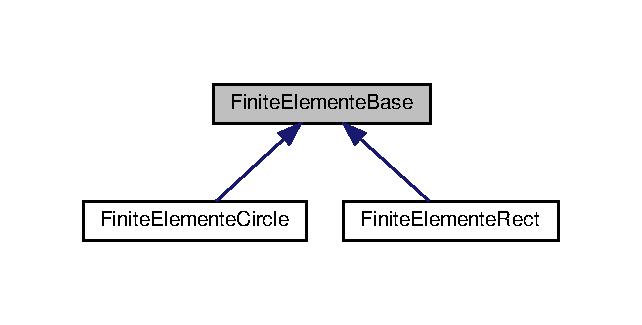
\includegraphics[width=308pt]{classFiniteElementeBase__inherit__graph}
\end{center}
\end{figure}
\subsection*{Public Member Functions}
\begin{DoxyCompactItemize}
\item 
\hyperlink{classFiniteElementeBase_a64ce4d3439a1ca2dfad3fdbe65f1b128}{Finite\+Elemente\+Base} (bool save\+Solution)
\item 
\mbox{\Hypertarget{classFiniteElementeBase_a75213fac01c8b3cd838d6cdcfcd45eb6}\label{classFiniteElementeBase_a75213fac01c8b3cd838d6cdcfcd45eb6}} 
void {\bfseries init\+Run} (bool init\+Device=false)
\item 
\mbox{\Hypertarget{classFiniteElementeBase_a0ae38114396c8676e1c2504f3e21f1c0}\label{classFiniteElementeBase_a0ae38114396c8676e1c2504f3e21f1c0}} 
void {\bfseries run} ()
\item 
\mbox{\Hypertarget{classFiniteElementeBase_a76778a3d7a97a6cb3121ac99ee232af2}\label{classFiniteElementeBase_a76778a3d7a97a6cb3121ac99ee232af2}} 
void {\bfseries update\+Electrode\+Voltage} (int const \&electrode\+Index, double const \&voltage)
\item 
virtual double \hyperlink{classFiniteElementeBase_aee384092436f2288ba1ceaf0f279afed}{get\+Potential} (double const \&x, double const \&y)
\item 
virtual void \hyperlink{classFiniteElementeBase_aff6763fa857bc57a629ef1c973fa5a49}{set\+Electrode} (double const \&voltage, double begin, double end)
\item 
virtual void \hyperlink{classFiniteElementeBase_abd7e36541ce728ab710166ab50fad93f}{set\+Electrode} (double const \&voltage, double begin, double end, int edge)
\end{DoxyCompactItemize}
\subsection*{Data Fields}
\begin{DoxyCompactItemize}
\item 
\mbox{\Hypertarget{classFiniteElementeBase_a0404964ec0d8191aba580cb49408c739}\label{classFiniteElementeBase_a0404964ec0d8191aba580cb49408c739}} 
Grid\+Function $\ast$ {\bfseries solution\+Vector}
\end{DoxyCompactItemize}
\subsection*{Protected Attributes}
\begin{DoxyCompactItemize}
\item 
\mbox{\Hypertarget{classFiniteElementeBase_a8ce243d0436c3a95ae35aba9ffdc52a7}\label{classFiniteElementeBase_a8ce243d0436c3a95ae35aba9ffdc52a7}} 
bool {\bfseries save\+Solution}
\item 
\mbox{\Hypertarget{classFiniteElementeBase_abe51bdeb3c0d4800d559aadca68e3766}\label{classFiniteElementeBase_abe51bdeb3c0d4800d559aadca68e3766}} 
int {\bfseries run\+Number} =0
\item 
\mbox{\Hypertarget{classFiniteElementeBase_a22655271a630485ae93a5ac236797ea6}\label{classFiniteElementeBase_a22655271a630485ae93a5ac236797ea6}} 
int const {\bfseries dim} = 2
\item 
\mbox{\Hypertarget{classFiniteElementeBase_ab1bc15c8fe252733b46e864237df1789}\label{classFiniteElementeBase_ab1bc15c8fe252733b46e864237df1789}} 
int const {\bfseries sdim} = 2
\item 
\mbox{\Hypertarget{classFiniteElementeBase_abb99e7c3a55eb43caf5079f87f60afd3}\label{classFiniteElementeBase_abb99e7c3a55eb43caf5079f87f60afd3}} 
int const {\bfseries order} =1
\item 
\mbox{\Hypertarget{classFiniteElementeBase_a266d74a52e8371f5c40ee8318bfc6823}\label{classFiniteElementeBase_a266d74a52e8371f5c40ee8318bfc6823}} 
std\+::vector$<$ std\+::vector$<$ int $>$ $>$ {\bfseries electrode\+Vertex\+Indices}
\item 
\mbox{\Hypertarget{classFiniteElementeBase_ad2d47704e683cbe72d8d7c5a2d35d01e}\label{classFiniteElementeBase_ad2d47704e683cbe72d8d7c5a2d35d01e}} 
int {\bfseries number\+Of\+Electrodes} =0
\item 
\mbox{\Hypertarget{classFiniteElementeBase_a2a563d27f0c4c717aaf06d93260eb973}\label{classFiniteElementeBase_a2a563d27f0c4c717aaf06d93260eb973}} 
Mesh $\ast$ {\bfseries mesh}
\item 
\mbox{\Hypertarget{classFiniteElementeBase_a69a18f1e5f57ed3aaa01abe40962d059}\label{classFiniteElementeBase_a69a18f1e5f57ed3aaa01abe40962d059}} 
Finite\+Element\+Collection $\ast$ {\bfseries fec}
\item 
\mbox{\Hypertarget{classFiniteElementeBase_af2f045aa62007d632ddac54ccecb8f7a}\label{classFiniteElementeBase_af2f045aa62007d632ddac54ccecb8f7a}} 
Finite\+Element\+Space $\ast$ {\bfseries fespace}
\item 
\mbox{\Hypertarget{classFiniteElementeBase_a7b4469156230281c1dcfaa440eb58d92}\label{classFiniteElementeBase_a7b4469156230281c1dcfaa440eb58d92}} 
Bilinear\+Form $\ast$ {\bfseries a}
\item 
\mbox{\Hypertarget{classFiniteElementeBase_a475862c154248228908de08499e67de0}\label{classFiniteElementeBase_a475862c154248228908de08499e67de0}} 
Linear\+Form $\ast$ {\bfseries b}
\item 
\mbox{\Hypertarget{classFiniteElementeBase_a9577bdbdb32662095d3d42865829a32f}\label{classFiniteElementeBase_a9577bdbdb32662095d3d42865829a32f}} 
Operator\+Ptr {\bfseries A}
\item 
\mbox{\Hypertarget{classFiniteElementeBase_a05338aab755f3c4e68f82d9cd4c42ccc}\label{classFiniteElementeBase_a05338aab755f3c4e68f82d9cd4c42ccc}} 
Vector {\bfseries B}
\item 
\mbox{\Hypertarget{classFiniteElementeBase_a397e8adff87d82c58905df0162e8cdd8}\label{classFiniteElementeBase_a397e8adff87d82c58905df0162e8cdd8}} 
Vector {\bfseries X}
\item 
\mbox{\Hypertarget{classFiniteElementeBase_aaaf65fe06be3766f539f0cc4616b7277}\label{classFiniteElementeBase_aaaf65fe06be3766f539f0cc4616b7277}} 
G\+S\+Smoother {\bfseries M}
\item 
\mbox{\Hypertarget{classFiniteElementeBase_a3d4eb8b924a21d426f0b07622f0e21eb}\label{classFiniteElementeBase_a3d4eb8b924a21d426f0b07622f0e21eb}} 
Array$<$ int $>$ {\bfseries ess\+\_\+tdof\+\_\+list}
\end{DoxyCompactItemize}


\subsection{Detailed Description}
Class to solve laplace equation. Parent class istself cant run, only childs. Analogously implemented to \href{https://github.com/mfem/mfem/blob/master/examples/ex1.cpp}{\tt https\+://github.\+com/mfem/mfem/blob/master/examples/ex1.\+cpp}. 

\subsection{Constructor \& Destructor Documentation}
\mbox{\Hypertarget{classFiniteElementeBase_a64ce4d3439a1ca2dfad3fdbe65f1b128}\label{classFiniteElementeBase_a64ce4d3439a1ca2dfad3fdbe65f1b128}} 
\index{Finite\+Elemente\+Base@{Finite\+Elemente\+Base}!Finite\+Elemente\+Base@{Finite\+Elemente\+Base}}
\index{Finite\+Elemente\+Base@{Finite\+Elemente\+Base}!Finite\+Elemente\+Base@{Finite\+Elemente\+Base}}
\subsubsection{\texorpdfstring{Finite\+Elemente\+Base()}{FiniteElementeBase()}}
{\footnotesize\ttfamily Finite\+Elemente\+Base\+::\+Finite\+Elemente\+Base (\begin{DoxyParamCaption}\item[{bool}]{save\+Solution }\end{DoxyParamCaption})}


\begin{DoxyParams}{Parameters}
{\em save\+Solution} & if true\+: save mesh and solution in each step. can be visualized using \char`\"{}glivs -\/m fin\+Ele.\+mesh -\/g laplace\+\_\+solution0.\+gf\char`\"{} \\
\hline
\end{DoxyParams}


\subsection{Member Function Documentation}
\mbox{\Hypertarget{classFiniteElementeBase_aee384092436f2288ba1ceaf0f279afed}\label{classFiniteElementeBase_aee384092436f2288ba1ceaf0f279afed}} 
\index{Finite\+Elemente\+Base@{Finite\+Elemente\+Base}!get\+Potential@{get\+Potential}}
\index{get\+Potential@{get\+Potential}!Finite\+Elemente\+Base@{Finite\+Elemente\+Base}}
\subsubsection{\texorpdfstring{get\+Potential()}{getPotential()}}
{\footnotesize\ttfamily virtual double Finite\+Elemente\+Base\+::get\+Potential (\begin{DoxyParamCaption}\item[{double const \&}]{x,  }\item[{double const \&}]{y }\end{DoxyParamCaption})\hspace{0.3cm}{\ttfamily [inline]}, {\ttfamily [virtual]}}

Get Potential using nearest neighbour interpolation 
\begin{DoxyParams}{Parameters}
{\em x} & in length units \\
\hline
{\em y} & in length units \\
\hline
\end{DoxyParams}


Reimplemented in \hyperlink{classFiniteElementeCircle_a832520dcd5db9bd2845ad3c781749a69}{Finite\+Elemente\+Circle}, and \hyperlink{classFiniteElementeRect_acbfa1b0263e192b4b7da51a486b623cf}{Finite\+Elemente\+Rect}.

\mbox{\Hypertarget{classFiniteElementeBase_aff6763fa857bc57a629ef1c973fa5a49}\label{classFiniteElementeBase_aff6763fa857bc57a629ef1c973fa5a49}} 
\index{Finite\+Elemente\+Base@{Finite\+Elemente\+Base}!set\+Electrode@{set\+Electrode}}
\index{set\+Electrode@{set\+Electrode}!Finite\+Elemente\+Base@{Finite\+Elemente\+Base}}
\subsubsection{\texorpdfstring{set\+Electrode()}{setElectrode()}\hspace{0.1cm}{\footnotesize\ttfamily [1/2]}}
{\footnotesize\ttfamily virtual void Finite\+Elemente\+Base\+::set\+Electrode (\begin{DoxyParamCaption}\item[{double const \&}]{voltage,  }\item[{double}]{begin,  }\item[{double}]{end }\end{DoxyParamCaption})\hspace{0.3cm}{\ttfamily [inline]}, {\ttfamily [virtual]}}

Set electrode position and voltage (boundary condition of laplace equation), polar version. 
\begin{DoxyParams}{Parameters}
{\em voltage} & in volts \\
\hline
{\em begin} & in radiant \\
\hline
{\em end} & in radiant \\
\hline
\end{DoxyParams}


Reimplemented in \hyperlink{classFiniteElementeCircle_aa3b2b0e50ab5ba53431bdc80674ead26}{Finite\+Elemente\+Circle}.

\mbox{\Hypertarget{classFiniteElementeBase_abd7e36541ce728ab710166ab50fad93f}\label{classFiniteElementeBase_abd7e36541ce728ab710166ab50fad93f}} 
\index{Finite\+Elemente\+Base@{Finite\+Elemente\+Base}!set\+Electrode@{set\+Electrode}}
\index{set\+Electrode@{set\+Electrode}!Finite\+Elemente\+Base@{Finite\+Elemente\+Base}}
\subsubsection{\texorpdfstring{set\+Electrode()}{setElectrode()}\hspace{0.1cm}{\footnotesize\ttfamily [2/2]}}
{\footnotesize\ttfamily virtual void Finite\+Elemente\+Base\+::set\+Electrode (\begin{DoxyParamCaption}\item[{double const \&}]{voltage,  }\item[{double}]{begin,  }\item[{double}]{end,  }\item[{int}]{edge }\end{DoxyParamCaption})\hspace{0.3cm}{\ttfamily [inline]}, {\ttfamily [virtual]}}

Set electrode position and voltage (boundary condition of laplace equation), cartesian version. 
\begin{DoxyParams}{Parameters}
{\em voltage} & in volts \\
\hline
{\em begin} & in length units \\
\hline
{\em end} & in length units \\
\hline
{\em edge} & see \hyperlink{structElectrodeParameters_a2f4cf737b66dcd4c7b74a836c9153918}{Electrode\+Parameters\+::edge} \\
\hline
\end{DoxyParams}


Reimplemented in \hyperlink{classFiniteElementeRect_a1b0c2fd8cc32d3bc9a23931f86b09406}{Finite\+Elemente\+Rect}.



The documentation for this class was generated from the following files\+:\begin{DoxyCompactItemize}
\item 
/home/marlon/\+Documents/\+Uni/master\+Chemie/\+M\+C\+Network/lib/finite\+Elemente/finite\+Elemente.\+h\item 
/home/marlon/\+Documents/\+Uni/master\+Chemie/\+M\+C\+Network/lib/finite\+Elemente/finite\+Elemente.\+cpp\end{DoxyCompactItemize}

\hypertarget{classFiniteElementeCircle}{}\section{Finite\+Elemente\+Circle Class Reference}
\label{classFiniteElementeCircle}\index{Finite\+Elemente\+Circle@{Finite\+Elemente\+Circle}}


Inheritance diagram for Finite\+Elemente\+Circle\+:\nopagebreak
\begin{figure}[H]
\begin{center}
\leavevmode
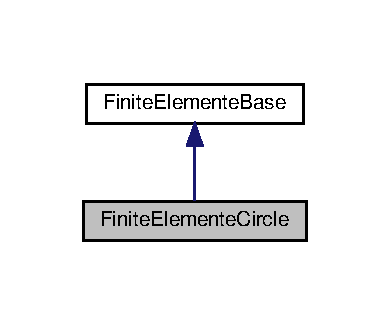
\includegraphics[width=187pt]{classFiniteElementeCircle__inherit__graph}
\end{center}
\end{figure}


Collaboration diagram for Finite\+Elemente\+Circle\+:\nopagebreak
\begin{figure}[H]
\begin{center}
\leavevmode
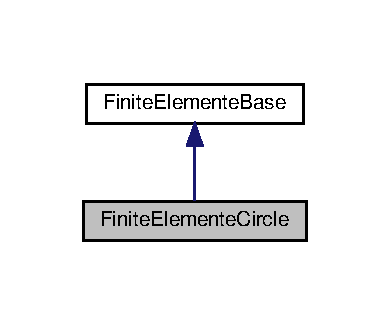
\includegraphics[width=187pt]{classFiniteElementeCircle__coll__graph}
\end{center}
\end{figure}
\subsection*{Public Member Functions}
\begin{DoxyCompactItemize}
\item 
\mbox{\Hypertarget{classFiniteElementeCircle_aef00567cba0a679abd3dee1c26b91c8b}\label{classFiniteElementeCircle_aef00567cba0a679abd3dee1c26b91c8b}} 
{\bfseries Finite\+Elemente\+Circle} (double const \&radius, int const \&max\+Number\+Of\+Elments, bool save\+Solution=false)
\item 
void \hyperlink{classFiniteElementeCircle_aa3b2b0e50ab5ba53431bdc80674ead26}{set\+Electrode} (double const \&voltage, double begin, double end)
\item 
double \hyperlink{classFiniteElementeCircle_a832520dcd5db9bd2845ad3c781749a69}{get\+Potential} (double const \&x, double const \&y)
\end{DoxyCompactItemize}
\subsection*{Private Member Functions}
\begin{DoxyCompactItemize}
\item 
\mbox{\Hypertarget{classFiniteElementeCircle_a479d6d3986a14d7011c3fa68a954d13b}\label{classFiniteElementeCircle_a479d6d3986a14d7011c3fa68a954d13b}} 
void {\bfseries init\+Mesh} (int const \&max\+Number\+Of\+Elements)
\end{DoxyCompactItemize}
\subsection*{Private Attributes}
\begin{DoxyCompactItemize}
\item 
\mbox{\Hypertarget{classFiniteElementeCircle_a9a16f2a7c9383994e39932eaff07e9a0}\label{classFiniteElementeCircle_a9a16f2a7c9383994e39932eaff07e9a0}} 
double const {\bfseries radius} = 0
\item 
\mbox{\Hypertarget{classFiniteElementeCircle_ac7e96d30db2e6f97c43cde584d42cb76}\label{classFiniteElementeCircle_ac7e96d30db2e6f97c43cde584d42cb76}} 
double {\bfseries deltaR}
\item 
\mbox{\Hypertarget{classFiniteElementeCircle_a2541895ba79ed701ee3b860f6a252e1e}\label{classFiniteElementeCircle_a2541895ba79ed701ee3b860f6a252e1e}} 
int {\bfseries layers}
\end{DoxyCompactItemize}
\subsection*{Additional Inherited Members}


\subsection{Member Function Documentation}
\mbox{\Hypertarget{classFiniteElementeCircle_a832520dcd5db9bd2845ad3c781749a69}\label{classFiniteElementeCircle_a832520dcd5db9bd2845ad3c781749a69}} 
\index{Finite\+Elemente\+Circle@{Finite\+Elemente\+Circle}!get\+Potential@{get\+Potential}}
\index{get\+Potential@{get\+Potential}!Finite\+Elemente\+Circle@{Finite\+Elemente\+Circle}}
\subsubsection{\texorpdfstring{get\+Potential()}{getPotential()}}
{\footnotesize\ttfamily double Finite\+Elemente\+Circle\+::get\+Potential (\begin{DoxyParamCaption}\item[{double const \&}]{x,  }\item[{double const \&}]{y }\end{DoxyParamCaption})\hspace{0.3cm}{\ttfamily [virtual]}}

Get Potential using nearest neighbour interpolation 
\begin{DoxyParams}{Parameters}
{\em x} & in length units \\
\hline
{\em y} & in length units \\
\hline
\end{DoxyParams}


Reimplemented from \hyperlink{classFiniteElementeBase_aee384092436f2288ba1ceaf0f279afed}{Finite\+Elemente\+Base}.

\mbox{\Hypertarget{classFiniteElementeCircle_aa3b2b0e50ab5ba53431bdc80674ead26}\label{classFiniteElementeCircle_aa3b2b0e50ab5ba53431bdc80674ead26}} 
\index{Finite\+Elemente\+Circle@{Finite\+Elemente\+Circle}!set\+Electrode@{set\+Electrode}}
\index{set\+Electrode@{set\+Electrode}!Finite\+Elemente\+Circle@{Finite\+Elemente\+Circle}}
\subsubsection{\texorpdfstring{set\+Electrode()}{setElectrode()}}
{\footnotesize\ttfamily void Finite\+Elemente\+Circle\+::set\+Electrode (\begin{DoxyParamCaption}\item[{double const \&}]{voltage,  }\item[{double}]{begin,  }\item[{double}]{end }\end{DoxyParamCaption})\hspace{0.3cm}{\ttfamily [virtual]}}

Set electrode position and voltage (boundary condition of laplace equation), polar version. 
\begin{DoxyParams}{Parameters}
{\em voltage} & in volts \\
\hline
{\em begin} & in radiant \\
\hline
{\em end} & in radiant \\
\hline
\end{DoxyParams}


Reimplemented from \hyperlink{classFiniteElementeBase_aff6763fa857bc57a629ef1c973fa5a49}{Finite\+Elemente\+Base}.



The documentation for this class was generated from the following files\+:\begin{DoxyCompactItemize}
\item 
/home/marlon/\+Documents/\+Uni/master\+Chemie/\+M\+C\+Network/lib/finite\+Elemente/finite\+Elemente.\+h\item 
/home/marlon/\+Documents/\+Uni/master\+Chemie/\+M\+C\+Network/lib/finite\+Elemente/finite\+Elemente.\+cpp\end{DoxyCompactItemize}

\hypertarget{classFiniteElementeRect}{}\section{Finite\+Elemente\+Rect Class Reference}
\label{classFiniteElementeRect}\index{Finite\+Elemente\+Rect@{Finite\+Elemente\+Rect}}


Inheritance diagram for Finite\+Elemente\+Rect\+:\nopagebreak
\begin{figure}[H]
\begin{center}
\leavevmode
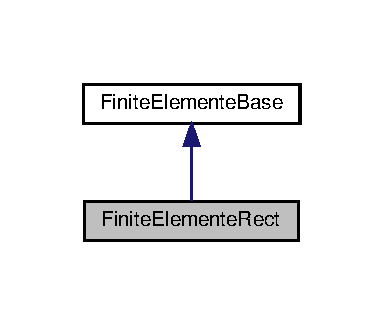
\includegraphics[width=184pt]{classFiniteElementeRect__inherit__graph}
\end{center}
\end{figure}


Collaboration diagram for Finite\+Elemente\+Rect\+:\nopagebreak
\begin{figure}[H]
\begin{center}
\leavevmode
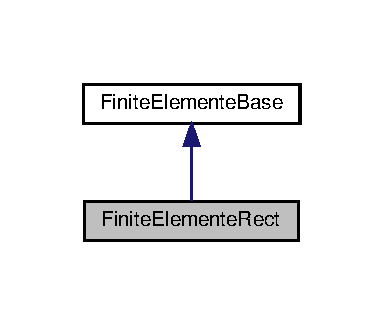
\includegraphics[width=184pt]{classFiniteElementeRect__coll__graph}
\end{center}
\end{figure}
\subsection*{Public Member Functions}
\begin{DoxyCompactItemize}
\item 
\mbox{\Hypertarget{classFiniteElementeRect_a5731bd88a8d13f73635015294042ab46}\label{classFiniteElementeRect_a5731bd88a8d13f73635015294042ab46}} 
{\bfseries Finite\+Elemente\+Rect} (double const \&len, double const \&width, int const \&max\+Number\+Of\+Elments, bool save\+Solution=false)
\item 
void \hyperlink{classFiniteElementeRect_a1b0c2fd8cc32d3bc9a23931f86b09406}{set\+Electrode} (double const \&voltage, double begin, double end, int edge)
\item 
double \hyperlink{classFiniteElementeRect_acbfa1b0263e192b4b7da51a486b623cf}{get\+Potential} (double const \&x, double const \&y)
\end{DoxyCompactItemize}
\subsection*{Private Member Functions}
\begin{DoxyCompactItemize}
\item 
\mbox{\Hypertarget{classFiniteElementeRect_a29ed0ced33fee536bcc8456e57094865}\label{classFiniteElementeRect_a29ed0ced33fee536bcc8456e57094865}} 
void {\bfseries init\+Mesh} (int const \&max\+Number\+Of\+Elements)
\end{DoxyCompactItemize}
\subsection*{Private Attributes}
\begin{DoxyCompactItemize}
\item 
\mbox{\Hypertarget{classFiniteElementeRect_a6beb13ebf0746380af8182e73ea1e929}\label{classFiniteElementeRect_a6beb13ebf0746380af8182e73ea1e929}} 
double const {\bfseries len} = 0
\item 
\mbox{\Hypertarget{classFiniteElementeRect_a88234e0caad5bdc5864fd210f4293719}\label{classFiniteElementeRect_a88234e0caad5bdc5864fd210f4293719}} 
double const {\bfseries width} = 0
\item 
\mbox{\Hypertarget{classFiniteElementeRect_a5bc6d292f48b09aaee773f03f7284f9e}\label{classFiniteElementeRect_a5bc6d292f48b09aaee773f03f7284f9e}} 
int {\bfseries number\+VerticesX}
\item 
\mbox{\Hypertarget{classFiniteElementeRect_a0609adb0d65d9aad1a9d566056838be3}\label{classFiniteElementeRect_a0609adb0d65d9aad1a9d566056838be3}} 
int {\bfseries number\+VerticesY}
\item 
\mbox{\Hypertarget{classFiniteElementeRect_a00313900e5e6bc821ddb74cff3349210}\label{classFiniteElementeRect_a00313900e5e6bc821ddb74cff3349210}} 
int $\ast$$\ast$ {\bfseries vertex\+Index\+Map}
\end{DoxyCompactItemize}
\subsection*{Additional Inherited Members}


\subsection{Member Function Documentation}
\mbox{\Hypertarget{classFiniteElementeRect_acbfa1b0263e192b4b7da51a486b623cf}\label{classFiniteElementeRect_acbfa1b0263e192b4b7da51a486b623cf}} 
\index{Finite\+Elemente\+Rect@{Finite\+Elemente\+Rect}!get\+Potential@{get\+Potential}}
\index{get\+Potential@{get\+Potential}!Finite\+Elemente\+Rect@{Finite\+Elemente\+Rect}}
\subsubsection{\texorpdfstring{get\+Potential()}{getPotential()}}
{\footnotesize\ttfamily double Finite\+Elemente\+Rect\+::get\+Potential (\begin{DoxyParamCaption}\item[{double const \&}]{x,  }\item[{double const \&}]{y }\end{DoxyParamCaption})\hspace{0.3cm}{\ttfamily [virtual]}}

Get Potential using nearest neighbour interpolation 
\begin{DoxyParams}{Parameters}
{\em x} & in length units \\
\hline
{\em y} & in length units \\
\hline
\end{DoxyParams}


Reimplemented from \hyperlink{classFiniteElementeBase_aee384092436f2288ba1ceaf0f279afed}{Finite\+Elemente\+Base}.

\mbox{\Hypertarget{classFiniteElementeRect_a1b0c2fd8cc32d3bc9a23931f86b09406}\label{classFiniteElementeRect_a1b0c2fd8cc32d3bc9a23931f86b09406}} 
\index{Finite\+Elemente\+Rect@{Finite\+Elemente\+Rect}!set\+Electrode@{set\+Electrode}}
\index{set\+Electrode@{set\+Electrode}!Finite\+Elemente\+Rect@{Finite\+Elemente\+Rect}}
\subsubsection{\texorpdfstring{set\+Electrode()}{setElectrode()}}
{\footnotesize\ttfamily void Finite\+Elemente\+Rect\+::set\+Electrode (\begin{DoxyParamCaption}\item[{double const \&}]{voltage,  }\item[{double}]{begin,  }\item[{double}]{end,  }\item[{int}]{edge }\end{DoxyParamCaption})\hspace{0.3cm}{\ttfamily [virtual]}}

Set electrode position and voltage (boundary condition of laplace equation), cartesian version. 
\begin{DoxyParams}{Parameters}
{\em voltage} & in volts \\
\hline
{\em begin} & in length units \\
\hline
{\em end} & in length units \\
\hline
{\em edge} & see \hyperlink{structElectrodeParameters_a2f4cf737b66dcd4c7b74a836c9153918}{Electrode\+Parameters\+::edge} \\
\hline
\end{DoxyParams}


Reimplemented from \hyperlink{classFiniteElementeBase_abd7e36541ce728ab710166ab50fad93f}{Finite\+Elemente\+Base}.



The documentation for this class was generated from the following files\+:\begin{DoxyCompactItemize}
\item 
/home/marlon/\+Documents/\+Uni/master\+Chemie/\+M\+C\+Network/lib/finite\+Elemente/finite\+Elemente.\+h\item 
/home/marlon/\+Documents/\+Uni/master\+Chemie/\+M\+C\+Network/lib/finite\+Elemente/finite\+Elemente.\+cpp\end{DoxyCompactItemize}

\hypertarget{classJob}{}\section{Job Class Reference}
\label{classJob}\index{Job@{Job}}


{\ttfamily \#include $<$jobhandling.\+h$>$}

\subsection*{Public Member Functions}
\begin{DoxyCompactItemize}
\item 
\mbox{\Hypertarget{classJob_ac7bd0c01cf61901df90b062f9a32cf02}\label{classJob_ac7bd0c01cf61901df90b062f9a32cf02}} 
{\bfseries Job} (int ID)
\end{DoxyCompactItemize}
\subsection*{Data Fields}
\begin{DoxyCompactItemize}
\item 
\mbox{\Hypertarget{classJob_a57ddffae23fca72e95103d4bf43c2809}\label{classJob_a57ddffae23fca72e95103d4bf43c2809}} 
int {\bfseries ID}
\item 
\mbox{\Hypertarget{classJob_ad0d1483df629cd0a619bb7fd6cc48a96}\label{classJob_ad0d1483df629cd0a619bb7fd6cc48a96}} 
std\+::unique\+\_\+ptr$<$ std\+::mutex $>$ {\bfseries job\+Mutex}
\item 
mfem\+::\+Grid\+Function \hyperlink{classJob_ad2b87bb3cea36a711bf7aace2d0cb338}{potential}
\item 
std\+::vector$<$ bool $>$ \hyperlink{classJob_a0c4579b73aec5c6755f271d78a488ae6}{equil\+Occupation}
\item 
\mbox{\Hypertarget{classJob_a0de73890acdd2d418ba26eceffbb160c}\label{classJob_a0de73890acdd2d418ba26eceffbb160c}} 
int {\bfseries equil\+Steps}
\item 
\mbox{\Hypertarget{classJob_a566a266e422eff68dfdae3e815d30dce}\label{classJob_a566a266e422eff68dfdae3e815d30dce}} 
int {\bfseries total\+Steps}
\item 
\mbox{\Hypertarget{classJob_ace6400f6ae321b8043b055128709644d}\label{classJob_ace6400f6ae321b8043b055128709644d}} 
int {\bfseries steps\+Per\+Task}
\item 
\mbox{\Hypertarget{classJob_a52154a755a4faa7b3804ca3c3b32e8bb}\label{classJob_a52154a755a4faa7b3804ca3c3b32e8bb}} 
int {\bfseries tasks\+To\+Go}
\item 
int \hyperlink{classJob_ae1cfd5a6e867f3664c8f183427a4775a}{thread\+Number} = 0
\item 
\mbox{\Hypertarget{classJob_af6d86a485ae26abfcdbe130fcd4ede85}\label{classJob_af6d86a485ae26abfcdbe130fcd4ede85}} 
std\+::vector$<$ double $>$ {\bfseries voltages}
\item 
\mbox{\Hypertarget{classJob_a1bb677c94a543ba9c4f4733d8ac4f948}\label{classJob_a1bb677c94a543ba9c4f4733d8ac4f948}} 
double {\bfseries result\+Current} = 0
\item 
\mbox{\Hypertarget{classJob_a823bcf86102a4ae9f1c431734547bc62}\label{classJob_a823bcf86102a4ae9f1c431734547bc62}} 
double {\bfseries result\+Current\+Uncert} = 0
\end{DoxyCompactItemize}
\subsection*{Static Public Attributes}
\begin{DoxyCompactItemize}
\item 
\mbox{\Hypertarget{classJob_a6db936569b3ad8309a69c8024adb4e09}\label{classJob_a6db936569b3ad8309a69c8024adb4e09}} 
static const int {\bfseries tasks\+Per\+Job} = 100
\end{DoxyCompactItemize}


\subsection{Detailed Description}
one job consits of one set of fixed voltages (incl. input voltages). steps to run are split up in tasks\+Per\+Job packs. each task can be handeled by single thread. 

\subsection{Field Documentation}
\mbox{\Hypertarget{classJob_a0c4579b73aec5c6755f271d78a488ae6}\label{classJob_a0c4579b73aec5c6755f271d78a488ae6}} 
\index{Job@{Job}!equil\+Occupation@{equil\+Occupation}}
\index{equil\+Occupation@{equil\+Occupation}!Job@{Job}}
\subsubsection{\texorpdfstring{equil\+Occupation}{equilOccupation}}
{\footnotesize\ttfamily std\+::vector$<$bool$>$ Job\+::equil\+Occupation}

equilibrium occupation of system. calculated only once by first thread and saved to pass it to other threads that might join work on this job \mbox{\Hypertarget{classJob_ad2b87bb3cea36a711bf7aace2d0cb338}\label{classJob_ad2b87bb3cea36a711bf7aace2d0cb338}} 
\index{Job@{Job}!potential@{potential}}
\index{potential@{potential}!Job@{Job}}
\subsubsection{\texorpdfstring{potential}{potential}}
{\footnotesize\ttfamily mfem\+::\+Grid\+Function Job\+::potential}

solution of laplace eq. calculated only once by first thread and saved to pass it to other threads that might join work on this job \mbox{\Hypertarget{classJob_ae1cfd5a6e867f3664c8f183427a4775a}\label{classJob_ae1cfd5a6e867f3664c8f183427a4775a}} 
\index{Job@{Job}!thread\+Number@{thread\+Number}}
\index{thread\+Number@{thread\+Number}!Job@{Job}}
\subsubsection{\texorpdfstring{thread\+Number}{threadNumber}}
{\footnotesize\ttfamily int Job\+::thread\+Number = 0}

number of threads that are currently working on this job 

The documentation for this class was generated from the following file\+:\begin{DoxyCompactItemize}
\item 
/home/marlon/\+Documents/\+Uni/master\+Chemie/\+M\+C\+Network/src/system/jobhandling.\+h\end{DoxyCompactItemize}

\hypertarget{classJobManager}{}\section{Job\+Manager Class Reference}
\label{classJobManager}\index{Job\+Manager@{Job\+Manager}}


{\ttfamily \#include $<$jobhandling.\+h$>$}

\subsection*{Public Member Functions}
\begin{DoxyCompactItemize}
\item 
\mbox{\Hypertarget{classJobManager_aa6b79c585bb341aec9f8ad384929c4d7}\label{classJobManager_aa6b79c585bb341aec9f8ad384929c4d7}} 
{\bfseries Job\+Manager} (std\+::shared\+\_\+ptr$<$ \hyperlink{classParameterStorage}{Parameter\+Storage} $>$)
\item 
std\+::pair$<$ std\+::vector$<$ double $>$, std\+::vector$<$ double $>$ $>$ const \hyperlink{classJobManager_af1a851cbf0d447aa2248a2d89b544e9d}{run\+Control\+Voltages\+Setup} (std\+::vector$<$ double $>$ const \&voltages)
\end{DoxyCompactItemize}
\subsection*{Static Private Member Functions}
\begin{DoxyCompactItemize}
\item 
static void \hyperlink{classJobManager_a478365d6287e01484a64105dcd81520e}{handle\+Job\+List} (std\+::vector$<$ \hyperlink{classJob}{Job} $>$ \&jobs, \hyperlink{classSystem}{System} $\ast$const system, std\+::mutex \&search\+Mutex)
\end{DoxyCompactItemize}
\subsection*{Private Attributes}
\begin{DoxyCompactItemize}
\item 
\mbox{\Hypertarget{classJobManager_af8fb3e539eda8e070bdf903b6b334ef4}\label{classJobManager_af8fb3e539eda8e070bdf903b6b334ef4}} 
int {\bfseries voltage\+Scan\+Points}
\item 
\mbox{\Hypertarget{classJobManager_ac5920380c45cbf6ba669af6c36889955}\label{classJobManager_ac5920380c45cbf6ba669af6c36889955}} 
int {\bfseries electrode\+Number}
\item 
\mbox{\Hypertarget{classJobManager_a9b463168e9fb04ac4452081a5c481c56}\label{classJobManager_a9b463168e9fb04ac4452081a5c481c56}} 
std\+::shared\+\_\+ptr$<$ \hyperlink{classParameterStorage}{Parameter\+Storage} $>$ {\bfseries parameter\+Storage}
\item 
\mbox{\Hypertarget{classJobManager_a0d5c04f0837027d5601e6468ec4fcab5}\label{classJobManager_a0d5c04f0837027d5601e6468ec4fcab5}} 
std\+::vector$<$ \hyperlink{classSystem}{System} $\ast$$>$ {\bfseries systems}
\item 
\mbox{\Hypertarget{classJobManager_adeb38892b4b5728b24368f3362442d45}\label{classJobManager_adeb38892b4b5728b24368f3362442d45}} 
std\+::vector$<$ \hyperlink{classJob}{Job} $>$ {\bfseries jobs}
\item 
std\+::mutex \hyperlink{classJobManager_af64a4f6d4843c3d5ca12c801c25666ac}{job\+Search\+Mutex}
\end{DoxyCompactItemize}


\subsection{Detailed Description}
handler for parallelization. 

\subsection{Member Function Documentation}
\mbox{\Hypertarget{classJobManager_a478365d6287e01484a64105dcd81520e}\label{classJobManager_a478365d6287e01484a64105dcd81520e}} 
\index{Job\+Manager@{Job\+Manager}!handle\+Job\+List@{handle\+Job\+List}}
\index{handle\+Job\+List@{handle\+Job\+List}!Job\+Manager@{Job\+Manager}}
\subsubsection{\texorpdfstring{handle\+Job\+List()}{handleJobList()}}
{\footnotesize\ttfamily void Job\+Manager\+::handle\+Job\+List (\begin{DoxyParamCaption}\item[{std\+::vector$<$ \hyperlink{classJob}{Job} $>$ \&}]{jobs,  }\item[{\hyperlink{classSystem}{System} $\ast$const}]{system,  }\item[{std\+::mutex \&}]{search\+Mutex }\end{DoxyParamCaption})\hspace{0.3cm}{\ttfamily [static]}, {\ttfamily [private]}}

method passed to parallel threads.
\begin{DoxyEnumerate}
\item search jobs vector for job to work on
\item if first thread in job -\/$>$ solve laplace eq, run equil steps
\item run tasks
\item if last thread -\/$>$ finish job
\item repeat with 1. until all jobs done 
\end{DoxyEnumerate}\mbox{\Hypertarget{classJobManager_af1a851cbf0d447aa2248a2d89b544e9d}\label{classJobManager_af1a851cbf0d447aa2248a2d89b544e9d}} 
\index{Job\+Manager@{Job\+Manager}!run\+Control\+Voltages\+Setup@{run\+Control\+Voltages\+Setup}}
\index{run\+Control\+Voltages\+Setup@{run\+Control\+Voltages\+Setup}!Job\+Manager@{Job\+Manager}}
\subsubsection{\texorpdfstring{run\+Control\+Voltages\+Setup()}{runControlVoltagesSetup()}}
{\footnotesize\ttfamily std\+::pair$<$ std\+::vector$<$ double $>$, std\+::vector$<$ double $>$ $>$ const Job\+Manager\+::run\+Control\+Voltages\+Setup (\begin{DoxyParamCaption}\item[{std\+::vector$<$ double $>$ const \&}]{voltages }\end{DoxyParamCaption})}

returns curr, curr\+Uncert 

\subsection{Field Documentation}
\mbox{\Hypertarget{classJobManager_af64a4f6d4843c3d5ca12c801c25666ac}\label{classJobManager_af64a4f6d4843c3d5ca12c801c25666ac}} 
\index{Job\+Manager@{Job\+Manager}!job\+Search\+Mutex@{job\+Search\+Mutex}}
\index{job\+Search\+Mutex@{job\+Search\+Mutex}!Job\+Manager@{Job\+Manager}}
\subsubsection{\texorpdfstring{job\+Search\+Mutex}{jobSearchMutex}}
{\footnotesize\ttfamily std\+::mutex Job\+Manager\+::job\+Search\+Mutex\hspace{0.3cm}{\ttfamily [private]}}

its only allowed to one thread at a time to search for new work! 

The documentation for this class was generated from the following files\+:\begin{DoxyCompactItemize}
\item 
/home/marlon/\+Documents/\+Uni/master\+Chemie/\+M\+C\+Network/src/system/jobhandling.\+h\item 
/home/marlon/\+Documents/\+Uni/master\+Chemie/\+M\+C\+Network/src/system/jobhandling.\+cpp\end{DoxyCompactItemize}

\hypertarget{classmyDebugger}{}\section{my\+Debugger Class Reference}
\label{classmyDebugger}\index{my\+Debugger@{my\+Debugger}}
\subsection*{Static Public Member Functions}
\begin{DoxyCompactItemize}
\item 
\mbox{\Hypertarget{classmyDebugger_ac32ad33ccc10846f7cd85881351197b5}\label{classmyDebugger_ac32ad33ccc10846f7cd85881351197b5}} 
static void {\bfseries debug\+Print} (std\+::string message, std\+::string key)
\end{DoxyCompactItemize}
\subsection*{Static Public Attributes}
\begin{DoxyCompactItemize}
\item 
\mbox{\Hypertarget{classmyDebugger_aa32856ddc22811f9754dc1f14bdbd859}\label{classmyDebugger_aa32856ddc22811f9754dc1f14bdbd859}} 
static int {\bfseries func\+Trace\+Level} =-\/1
\item 
\mbox{\Hypertarget{classmyDebugger_afe246c9eead29364742fd5de3e245655}\label{classmyDebugger_afe246c9eead29364742fd5de3e245655}} 
static std\+::set$<$ std\+::string $>$ {\bfseries debug\+Keys} =\{\char`\"{}func\+Trace\char`\"{}\}
\end{DoxyCompactItemize}


The documentation for this class was generated from the following files\+:\begin{DoxyCompactItemize}
\item 
/home/marlon/\+Documents/\+Uni/master\+Chemie/\+M\+C\+Network/src/debug.\+h\item 
/home/marlon/\+Documents/\+Uni/master\+Chemie/\+M\+C\+Network/src/debug.\+cpp\end{DoxyCompactItemize}

\hypertarget{classOptimizer}{}\section{Optimizer Class Reference}
\label{classOptimizer}\index{Optimizer@{Optimizer}}


{\ttfamily \#include $<$optimizer.\+h$>$}



Collaboration diagram for Optimizer\+:\nopagebreak
\begin{figure}[H]
\begin{center}
\leavevmode
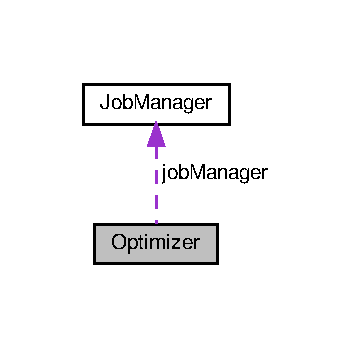
\includegraphics[width=169pt]{classOptimizer__coll__graph}
\end{center}
\end{figure}
\subsection*{Public Member Functions}
\begin{DoxyCompactItemize}
\item 
\mbox{\Hypertarget{classOptimizer_a60755ddbe7164fbee43ed25399613b9e}\label{classOptimizer_a60755ddbe7164fbee43ed25399613b9e}} 
{\bfseries Optimizer} (std\+::shared\+\_\+ptr$<$ \hyperlink{classParameterStorage}{Parameter\+Storage} $>$)
\item 
void \hyperlink{classOptimizer_aa9fdb7cd911fdd9fbfaf3fc8d86ea408}{run} (std\+::string \hyperlink{classOptimizer_aba4673e21bc48603b1acd38cfb01b422}{optimization\+Mode}, int start\+Mode)
\end{DoxyCompactItemize}
\subsection*{Private Member Functions}
\begin{DoxyCompactItemize}
\item 
void \hyperlink{classOptimizer_a82f53be5481740bf2cc2ff921af38a51}{calc\+Optimization\+Energy} ()
\item 
void \hyperlink{classOptimizer_a67407e1db0c02fa16ac4c6438dcd0e74}{save\+Results} (size\+\_\+t index=0)
\item 
\mbox{\Hypertarget{classOptimizer_a92ae8533ed25af8f0071124913418ea9}\label{classOptimizer_a92ae8533ed25af8f0071124913418ea9}} 
bool {\bfseries desired\+Logic\+Function} (double val1, double val2, std\+::string gate)
\item 
void \hyperlink{classOptimizer_a5dfd9a3a649ffa7e064c49d00afdb384}{search\+For\+Random\+Start} ()
\item 
void \hyperlink{classOptimizer_aff5efd6e481349d870e12221ce865a25}{single\+Run} (size\+\_\+t start\+Mode=0)
\item 
void \hyperlink{classOptimizer_a70cfb2468659d3d06d2fb7ba959c1f67}{optimize\+MC} (size\+\_\+t start\+Mode=0)
\item 
void \hyperlink{classOptimizer_a927fdf3177a1e0479d2caf69af541c5d}{optimize\+Genetic} (size\+\_\+t start\+Mode=0)
\item 
void \hyperlink{classOptimizer_a53f16ba66dc160c7f7c8e27e8e3de90f}{optimize\+Basin\+Hopping} (size\+\_\+t start\+Mode=0)
\item 
void \hyperlink{classOptimizer_a29a003cd019aa5908d1bb2bd317b1589}{optimize\+Gradient} ()
\item 
void \hyperlink{classOptimizer_accdf2a36a2b565ec87f5a251c970520e}{continue\+Simulation} ()
\end{DoxyCompactItemize}
\subsection*{Private Attributes}
\begin{DoxyCompactItemize}
\item 
int \hyperlink{classOptimizer_a291e98d2c2f585d0076df4eeb04878e5}{electrode\+Number}
\item 
int \hyperlink{classOptimizer_a884c041fbb25a872c72b5062823180b1}{voltage\+Scan\+Points}
\item 
size\+\_\+t \hyperlink{classOptimizer_afa7c063bddb3580a06a62642a3fe2e86}{control\+Electrode\+Number}
\item 
double \hyperlink{classOptimizer_a81991596f83ec6ded5c3b45545cde3cd}{fitness} = 0
\item 
double \hyperlink{classOptimizer_a43a00ff6308575ffdea61f31b5c8bda0}{fitness\+Uncert} = 0
\item 
double \hyperlink{classOptimizer_aea24c0bcb76dfd328f6f21b18046891d}{opt\+Energy} = 0
\item 
double \hyperlink{classOptimizer_a30bba218ee4f03978b1b3358a8b3ea62}{normed\+Diff} = 0
\item 
\mbox{\Hypertarget{classOptimizer_a65468e1da4d3ffa58a9e1613b41702df}\label{classOptimizer_a65468e1da4d3ffa58a9e1613b41702df}} 
size\+\_\+t {\bfseries iteration} =0
\item 
size\+\_\+t \hyperlink{classOptimizer_a7b388654b13c174e265e81e949d5a69b}{last\+Iteration\+Increase} = 0
\item 
std\+::string \hyperlink{classOptimizer_aba4673e21bc48603b1acd38cfb01b422}{optimization\+Mode}
\item 
std\+::vector$<$ std\+::pair$<$ std\+::vector$<$ double $>$, double $>$ $>$ \hyperlink{classOptimizer_ac4668dd4b83b15cb877daa134f55e5e2}{voltage\+Energy\+Sets}
\item 
std\+::vector$<$ double $>$ \hyperlink{classOptimizer_af36d52fa81a2f38b5cb419e2c800fad6}{output\+Currents}
\item 
std\+::vector$<$ double $>$ \hyperlink{classOptimizer_a65b7546e16edb4ea05a041812590a873}{output\+Current\+Uncerts}
\item 
std\+::vector$<$ size\+\_\+t $>$ \hyperlink{classOptimizer_a0204c3a84115d2ca60ac03b1e08f6db2}{control\+Electrode\+Indices}
\item 
\mbox{\Hypertarget{classOptimizer_adc47879768ab5fb34797f3f7f9628ae1}\label{classOptimizer_adc47879768ab5fb34797f3f7f9628ae1}} 
std\+::shared\+\_\+ptr$<$ \hyperlink{classParameterStorage}{Parameter\+Storage} $>$ {\bfseries parameter\+Storage}
\item 
\mbox{\Hypertarget{classOptimizer_a8c0dca31122f1c5abda3b85697922135}\label{classOptimizer_a8c0dca31122f1c5abda3b85697922135}} 
std\+::shared\+\_\+ptr$<$ \hyperlink{classDataFile}{Data\+File} $>$ {\bfseries data\+File}
\item 
std\+::shared\+\_\+ptr$<$ std\+::vector$<$ \hyperlink{classSystem}{System} $\ast$$>$ $>$ \hyperlink{classOptimizer_a73db0a3546c6d5fab4237de7dd961f89}{systems}
\item 
\mbox{\Hypertarget{classOptimizer_a63257684f09c2d4d53c85dfc463aa689}\label{classOptimizer_a63257684f09c2d4d53c85dfc463aa689}} 
\hyperlink{classJobManager}{Job\+Manager} {\bfseries job\+Manager}
\end{DoxyCompactItemize}


\subsection{Detailed Description}
container for optimization routines. 

\subsection{Member Function Documentation}
\mbox{\Hypertarget{classOptimizer_a82f53be5481740bf2cc2ff921af38a51}\label{classOptimizer_a82f53be5481740bf2cc2ff921af38a51}} 
\index{Optimizer@{Optimizer}!calc\+Optimization\+Energy@{calc\+Optimization\+Energy}}
\index{calc\+Optimization\+Energy@{calc\+Optimization\+Energy}!Optimizer@{Optimizer}}
\subsubsection{\texorpdfstring{calc\+Optimization\+Energy()}{calcOptimizationEnergy()}}
{\footnotesize\ttfamily void Optimizer\+::calc\+Optimization\+Energy (\begin{DoxyParamCaption}{ }\end{DoxyParamCaption})\hspace{0.3cm}{\ttfamily [private]}}

calc\+Optimization\+Energy using values stored in \hyperlink{classOptimizer_af36d52fa81a2f38b5cb419e2c800fad6}{Optimizer\+::output\+Currents} and \hyperlink{classOptimizer_a65b7546e16edb4ea05a041812590a873}{Optimizer\+::output\+Current\+Uncerts}. saves output to \hyperlink{classOptimizer_a81991596f83ec6ded5c3b45545cde3cd}{Optimizer\+::fitness}, \hyperlink{classOptimizer_a43a00ff6308575ffdea61f31b5c8bda0}{Optimizer\+::fitness\+Uncert}, \hyperlink{classOptimizer_a30bba218ee4f03978b1b3358a8b3ea62}{Optimizer\+::normed\+Diff}, \hyperlink{classOptimizer_aea24c0bcb76dfd328f6f21b18046891d}{Optimizer\+::opt\+Energy} 
\begin{DoxyParams}{Parameters}
{\em index} & determines which set stored in voltage\+Energy\+Sets shall be saved. default = 0. \\
\hline
\end{DoxyParams}
\mbox{\Hypertarget{classOptimizer_accdf2a36a2b565ec87f5a251c970520e}\label{classOptimizer_accdf2a36a2b565ec87f5a251c970520e}} 
\index{Optimizer@{Optimizer}!continue\+Simulation@{continue\+Simulation}}
\index{continue\+Simulation@{continue\+Simulation}!Optimizer@{Optimizer}}
\subsubsection{\texorpdfstring{continue\+Simulation()}{continueSimulation()}}
{\footnotesize\ttfamily void Optimizer\+::continue\+Simulation (\begin{DoxyParamCaption}{ }\end{DoxyParamCaption})\hspace{0.3cm}{\ttfamily [private]}}

is called by \hyperlink{classOptimizer_aa9fdb7cd911fdd9fbfaf3fc8d86ea408}{Optimizer\+::run} in case of \char`\"{}-\/-\/continue\char`\"{} option set. setup optimization parameters for continuation. \mbox{\Hypertarget{classOptimizer_a53f16ba66dc160c7f7c8e27e8e3de90f}\label{classOptimizer_a53f16ba66dc160c7f7c8e27e8e3de90f}} 
\index{Optimizer@{Optimizer}!optimize\+Basin\+Hopping@{optimize\+Basin\+Hopping}}
\index{optimize\+Basin\+Hopping@{optimize\+Basin\+Hopping}!Optimizer@{Optimizer}}
\subsubsection{\texorpdfstring{optimize\+Basin\+Hopping()}{optimizeBasinHopping()}}
{\footnotesize\ttfamily void Optimizer\+::optimize\+Basin\+Hopping (\begin{DoxyParamCaption}\item[{size\+\_\+t}]{start\+Mode = {\ttfamily 0} }\end{DoxyParamCaption})\hspace{0.3cm}{\ttfamily [private]}}

optimize cotrol voltages using basin hopping 
\begin{DoxyParams}{Parameters}
{\em rnd\+Start} & 0\+: \hyperlink{classOptimizer_a5dfd9a3a649ffa7e064c49d00afdb384}{search\+For\+Random\+Start()} is called to find best start point ~\newline
 1\+: voltages given in input file are used ~\newline
 2\+: used in continue mode, voltages have been set before \\
\hline
\end{DoxyParams}
\mbox{\Hypertarget{classOptimizer_a927fdf3177a1e0479d2caf69af541c5d}\label{classOptimizer_a927fdf3177a1e0479d2caf69af541c5d}} 
\index{Optimizer@{Optimizer}!optimize\+Genetic@{optimize\+Genetic}}
\index{optimize\+Genetic@{optimize\+Genetic}!Optimizer@{Optimizer}}
\subsubsection{\texorpdfstring{optimize\+Genetic()}{optimizeGenetic()}}
{\footnotesize\ttfamily void Optimizer\+::optimize\+Genetic (\begin{DoxyParamCaption}\item[{size\+\_\+t}]{start\+Mode = {\ttfamily 0} }\end{DoxyParamCaption})\hspace{0.3cm}{\ttfamily [private]}}

optimize cotrol voltages using genetic algorithm 
\begin{DoxyParams}{Parameters}
{\em rnd\+Start} & 0\+: \hyperlink{classOptimizer_a5dfd9a3a649ffa7e064c49d00afdb384}{search\+For\+Random\+Start()} is called to find best start point ~\newline
 1\+: voltages given in input file are used ~\newline
 2\+: used in continue mode, voltages have been set before \\
\hline
\end{DoxyParams}
$<$$<$$<$$<$ bug here\+: if k=14, k=5 is taken, but voltage\+Energy\+Sets\mbox{[}5\mbox{]} was overwritten before \mbox{\Hypertarget{classOptimizer_a29a003cd019aa5908d1bb2bd317b1589}\label{classOptimizer_a29a003cd019aa5908d1bb2bd317b1589}} 
\index{Optimizer@{Optimizer}!optimize\+Gradient@{optimize\+Gradient}}
\index{optimize\+Gradient@{optimize\+Gradient}!Optimizer@{Optimizer}}
\subsubsection{\texorpdfstring{optimize\+Gradient()}{optimizeGradient()}}
{\footnotesize\ttfamily void Optimizer\+::optimize\+Gradient (\begin{DoxyParamCaption}{ }\end{DoxyParamCaption})\hspace{0.3cm}{\ttfamily [private]}}

optimize cotrol voltages along the local gradient -\/ not implemented yet \mbox{\Hypertarget{classOptimizer_a70cfb2468659d3d06d2fb7ba959c1f67}\label{classOptimizer_a70cfb2468659d3d06d2fb7ba959c1f67}} 
\index{Optimizer@{Optimizer}!optimize\+MC@{optimize\+MC}}
\index{optimize\+MC@{optimize\+MC}!Optimizer@{Optimizer}}
\subsubsection{\texorpdfstring{optimize\+M\+C()}{optimizeMC()}}
{\footnotesize\ttfamily void Optimizer\+::optimize\+MC (\begin{DoxyParamCaption}\item[{size\+\_\+t}]{start\+Mode = {\ttfamily 0} }\end{DoxyParamCaption})\hspace{0.3cm}{\ttfamily [private]}}

optimize cotrol voltages using simple Monte Carlo algorithm 
\begin{DoxyParams}{Parameters}
{\em rnd\+Start} & 0\+: \hyperlink{classOptimizer_a5dfd9a3a649ffa7e064c49d00afdb384}{search\+For\+Random\+Start()} is called to find best start point ~\newline
 1\+: voltages given in input file are used ~\newline
 2\+: used in continue mode, voltages have been set before \\
\hline
\end{DoxyParams}
\mbox{\Hypertarget{classOptimizer_aa9fdb7cd911fdd9fbfaf3fc8d86ea408}\label{classOptimizer_aa9fdb7cd911fdd9fbfaf3fc8d86ea408}} 
\index{Optimizer@{Optimizer}!run@{run}}
\index{run@{run}!Optimizer@{Optimizer}}
\subsubsection{\texorpdfstring{run()}{run()}}
{\footnotesize\ttfamily void Optimizer\+::run (\begin{DoxyParamCaption}\item[{std\+::string}]{optimization\+Mode,  }\item[{int}]{start\+Mode }\end{DoxyParamCaption})}


\begin{DoxyItemize}
\item create datafile
\item start actual optimization routines 
\begin{DoxyParams}{Parameters}
{\em start\+Mode} & 0 = use voltages defined in input file, 1 = search for random start using \hyperlink{classOptimizer_a5dfd9a3a649ffa7e064c49d00afdb384}{search\+For\+Random\+Start()}, 2 = continue \\
\hline
\end{DoxyParams}

\end{DoxyItemize}\mbox{\Hypertarget{classOptimizer_a67407e1db0c02fa16ac4c6438dcd0e74}\label{classOptimizer_a67407e1db0c02fa16ac4c6438dcd0e74}} 
\index{Optimizer@{Optimizer}!save\+Results@{save\+Results}}
\index{save\+Results@{save\+Results}!Optimizer@{Optimizer}}
\subsubsection{\texorpdfstring{save\+Results()}{saveResults()}}
{\footnotesize\ttfamily void Optimizer\+::save\+Results (\begin{DoxyParamCaption}\item[{size\+\_\+t}]{index = {\ttfamily 0} }\end{DoxyParamCaption})\hspace{0.3cm}{\ttfamily [private]}}

saves following datsets to data\+File\+: Optimizer\+::output\+Current, Optimizer\+::output\+Current\+Uncert, Optimizer\+::voltages, \hyperlink{classOptimizer_a81991596f83ec6ded5c3b45545cde3cd}{Optimizer\+::fitness}, \hyperlink{classOptimizer_a43a00ff6308575ffdea61f31b5c8bda0}{Optimizer\+::fitness\+Uncert}, o\+Optimizer\+::pt\+Energy 
\begin{DoxyParams}{Parameters}
{\em index} & determines which set stored in \hyperlink{classOptimizer_ac4668dd4b83b15cb877daa134f55e5e2}{Optimizer\+::voltage\+Energy\+Sets} shall be saved. default = 0. \\
\hline
\end{DoxyParams}
\mbox{\Hypertarget{classOptimizer_a5dfd9a3a649ffa7e064c49d00afdb384}\label{classOptimizer_a5dfd9a3a649ffa7e064c49d00afdb384}} 
\index{Optimizer@{Optimizer}!search\+For\+Random\+Start@{search\+For\+Random\+Start}}
\index{search\+For\+Random\+Start@{search\+For\+Random\+Start}!Optimizer@{Optimizer}}
\subsubsection{\texorpdfstring{search\+For\+Random\+Start()}{searchForRandomStart()}}
{\footnotesize\ttfamily void Optimizer\+::search\+For\+Random\+Start (\begin{DoxyParamCaption}{ }\end{DoxyParamCaption})\hspace{0.3cm}{\ttfamily [private]}}

generates \char`\"{}rnd\+Start\+Points\char`\"{} random control voltage points and sets voltage\+Energy\+Sets\mbox{[}0\mbox{]} to the best result \mbox{\Hypertarget{classOptimizer_aff5efd6e481349d870e12221ce865a25}\label{classOptimizer_aff5efd6e481349d870e12221ce865a25}} 
\index{Optimizer@{Optimizer}!single\+Run@{single\+Run}}
\index{single\+Run@{single\+Run}!Optimizer@{Optimizer}}
\subsubsection{\texorpdfstring{single\+Run()}{singleRun()}}
{\footnotesize\ttfamily void Optimizer\+::single\+Run (\begin{DoxyParamCaption}\item[{size\+\_\+t}]{start\+Mode = {\ttfamily 0} }\end{DoxyParamCaption})\hspace{0.3cm}{\ttfamily [private]}}

not performing any optimization, just runing control voltages defined in input file 

\subsection{Field Documentation}
\mbox{\Hypertarget{classOptimizer_a0204c3a84115d2ca60ac03b1e08f6db2}\label{classOptimizer_a0204c3a84115d2ca60ac03b1e08f6db2}} 
\index{Optimizer@{Optimizer}!control\+Electrode\+Indices@{control\+Electrode\+Indices}}
\index{control\+Electrode\+Indices@{control\+Electrode\+Indices}!Optimizer@{Optimizer}}
\subsubsection{\texorpdfstring{control\+Electrode\+Indices}{controlElectrodeIndices}}
{\footnotesize\ttfamily std\+::vector$<$size\+\_\+t$>$ Optimizer\+::control\+Electrode\+Indices\hspace{0.3cm}{\ttfamily [private]}}

\mbox{[}i for i in range(electrode\+Number) if (i != output\+Electrode and i != input\+Electrode)\mbox{]} \mbox{\Hypertarget{classOptimizer_afa7c063bddb3580a06a62642a3fe2e86}\label{classOptimizer_afa7c063bddb3580a06a62642a3fe2e86}} 
\index{Optimizer@{Optimizer}!control\+Electrode\+Number@{control\+Electrode\+Number}}
\index{control\+Electrode\+Number@{control\+Electrode\+Number}!Optimizer@{Optimizer}}
\subsubsection{\texorpdfstring{control\+Electrode\+Number}{controlElectrodeNumber}}
{\footnotesize\ttfamily size\+\_\+t Optimizer\+::control\+Electrode\+Number\hspace{0.3cm}{\ttfamily [private]}}

number of control electrodes = electrode\+Number -\/ 3 \mbox{\Hypertarget{classOptimizer_a291e98d2c2f585d0076df4eeb04878e5}\label{classOptimizer_a291e98d2c2f585d0076df4eeb04878e5}} 
\index{Optimizer@{Optimizer}!electrode\+Number@{electrode\+Number}}
\index{electrode\+Number@{electrode\+Number}!Optimizer@{Optimizer}}
\subsubsection{\texorpdfstring{electrode\+Number}{electrodeNumber}}
{\footnotesize\ttfamily int Optimizer\+::electrode\+Number\hspace{0.3cm}{\ttfamily [private]}}

number of electrodes \mbox{\Hypertarget{classOptimizer_a81991596f83ec6ded5c3b45545cde3cd}\label{classOptimizer_a81991596f83ec6ded5c3b45545cde3cd}} 
\index{Optimizer@{Optimizer}!fitness@{fitness}}
\index{fitness@{fitness}!Optimizer@{Optimizer}}
\subsubsection{\texorpdfstring{fitness}{fitness}}
{\footnotesize\ttfamily double Optimizer\+::fitness = 0\hspace{0.3cm}{\ttfamily [private]}}

raw fitness \mbox{\Hypertarget{classOptimizer_a43a00ff6308575ffdea61f31b5c8bda0}\label{classOptimizer_a43a00ff6308575ffdea61f31b5c8bda0}} 
\index{Optimizer@{Optimizer}!fitness\+Uncert@{fitness\+Uncert}}
\index{fitness\+Uncert@{fitness\+Uncert}!Optimizer@{Optimizer}}
\subsubsection{\texorpdfstring{fitness\+Uncert}{fitnessUncert}}
{\footnotesize\ttfamily double Optimizer\+::fitness\+Uncert = 0\hspace{0.3cm}{\ttfamily [private]}}

uncertainty of raw fitness \mbox{\Hypertarget{classOptimizer_a7b388654b13c174e265e81e949d5a69b}\label{classOptimizer_a7b388654b13c174e265e81e949d5a69b}} 
\index{Optimizer@{Optimizer}!last\+Iteration\+Increase@{last\+Iteration\+Increase}}
\index{last\+Iteration\+Increase@{last\+Iteration\+Increase}!Optimizer@{Optimizer}}
\subsubsection{\texorpdfstring{last\+Iteration\+Increase}{lastIterationIncrease}}
{\footnotesize\ttfamily size\+\_\+t Optimizer\+::last\+Iteration\+Increase = 0\hspace{0.3cm}{\ttfamily [private]}}

only used in basin\+Hop mode. last time opt\+Energy increased \mbox{\Hypertarget{classOptimizer_a30bba218ee4f03978b1b3358a8b3ea62}\label{classOptimizer_a30bba218ee4f03978b1b3358a8b3ea62}} 
\index{Optimizer@{Optimizer}!normed\+Diff@{normed\+Diff}}
\index{normed\+Diff@{normed\+Diff}!Optimizer@{Optimizer}}
\subsubsection{\texorpdfstring{normed\+Diff}{normedDiff}}
{\footnotesize\ttfamily double Optimizer\+::normed\+Diff = 0\hspace{0.3cm}{\ttfamily [private]}}

parameter to quantify difference between high und low output current \mbox{\Hypertarget{classOptimizer_aea24c0bcb76dfd328f6f21b18046891d}\label{classOptimizer_aea24c0bcb76dfd328f6f21b18046891d}} 
\index{Optimizer@{Optimizer}!opt\+Energy@{opt\+Energy}}
\index{opt\+Energy@{opt\+Energy}!Optimizer@{Optimizer}}
\subsubsection{\texorpdfstring{opt\+Energy}{optEnergy}}
{\footnotesize\ttfamily double Optimizer\+::opt\+Energy = 0\hspace{0.3cm}{\ttfamily [private]}}

!! optimization energy is called \char`\"{}(corrected) fitness/ \textbackslash{}mathcal\{\+F\}\char`\"{} in thesis!!. optimization energy of last simulated voltage set. set by \hyperlink{classOptimizer_a82f53be5481740bf2cc2ff921af38a51}{calc\+Optimization\+Energy()}. only local variable, use voltage\+Energy\+Sets\mbox{[}i\mbox{]}.second instead. \mbox{\Hypertarget{classOptimizer_aba4673e21bc48603b1acd38cfb01b422}\label{classOptimizer_aba4673e21bc48603b1acd38cfb01b422}} 
\index{Optimizer@{Optimizer}!optimization\+Mode@{optimization\+Mode}}
\index{optimization\+Mode@{optimization\+Mode}!Optimizer@{Optimizer}}
\subsubsection{\texorpdfstring{optimization\+Mode}{optimizationMode}}
{\footnotesize\ttfamily std\+::string Optimizer\+::optimization\+Mode\hspace{0.3cm}{\ttfamily [private]}}

MC, genetic, basin\+Hop, single\+Run \mbox{\Hypertarget{classOptimizer_af36d52fa81a2f38b5cb419e2c800fad6}\label{classOptimizer_af36d52fa81a2f38b5cb419e2c800fad6}} 
\index{Optimizer@{Optimizer}!output\+Currents@{output\+Currents}}
\index{output\+Currents@{output\+Currents}!Optimizer@{Optimizer}}
\subsubsection{\texorpdfstring{output\+Currents}{outputCurrents}}
{\footnotesize\ttfamily std\+::vector$<$double$>$ Optimizer\+::output\+Currents\hspace{0.3cm}{\ttfamily [private]}}

output\+Currents for one set of control electrodes \mbox{\Hypertarget{classOptimizer_a65b7546e16edb4ea05a041812590a873}\label{classOptimizer_a65b7546e16edb4ea05a041812590a873}} 
\index{Optimizer@{Optimizer}!output\+Current\+Uncerts@{output\+Current\+Uncerts}}
\index{output\+Current\+Uncerts@{output\+Current\+Uncerts}!Optimizer@{Optimizer}}
\subsubsection{\texorpdfstring{output\+Current\+Uncerts}{outputCurrentUncerts}}
{\footnotesize\ttfamily std\+::vector$<$double$>$ Optimizer\+::output\+Current\+Uncerts\hspace{0.3cm}{\ttfamily [private]}}

output\+Current uncertainties for one set of control electrodes \mbox{\Hypertarget{classOptimizer_a73db0a3546c6d5fab4237de7dd961f89}\label{classOptimizer_a73db0a3546c6d5fab4237de7dd961f89}} 
\index{Optimizer@{Optimizer}!systems@{systems}}
\index{systems@{systems}!Optimizer@{Optimizer}}
\subsubsection{\texorpdfstring{systems}{systems}}
{\footnotesize\ttfamily std\+::shared\+\_\+ptr$<$std\+::vector$<$\hyperlink{classSystem}{System} $\ast$ $>$ $>$ Optimizer\+::systems\hspace{0.3cm}{\ttfamily [private]}}

multiple systems are created for parallelization and stored in shared pointer to be accessiable by job\+Maneger and optimizer \mbox{\Hypertarget{classOptimizer_ac4668dd4b83b15cb877daa134f55e5e2}\label{classOptimizer_ac4668dd4b83b15cb877daa134f55e5e2}} 
\index{Optimizer@{Optimizer}!voltage\+Energy\+Sets@{voltage\+Energy\+Sets}}
\index{voltage\+Energy\+Sets@{voltage\+Energy\+Sets}!Optimizer@{Optimizer}}
\subsubsection{\texorpdfstring{voltage\+Energy\+Sets}{voltageEnergySets}}
{\footnotesize\ttfamily std\+::vector$<$std\+::pair$<$std\+::vector$<$double$>$,double$>$ $>$ Optimizer\+::voltage\+Energy\+Sets\hspace{0.3cm}{\ttfamily [private]}}

all methods share one central storage for all sets of control voltages and corresponding opt\+Energies they need to know at a time. size and indexing differs from method to method, see methods doc for more details.~\newline
 voltage\+Energy\+Sets consists of pair of vector of control voltages and opt\+Energy. ~\newline
 first = voltages ~\newline
 second = opt\+Energy. \mbox{\Hypertarget{classOptimizer_a884c041fbb25a872c72b5062823180b1}\label{classOptimizer_a884c041fbb25a872c72b5062823180b1}} 
\index{Optimizer@{Optimizer}!voltage\+Scan\+Points@{voltage\+Scan\+Points}}
\index{voltage\+Scan\+Points@{voltage\+Scan\+Points}!Optimizer@{Optimizer}}
\subsubsection{\texorpdfstring{voltage\+Scan\+Points}{voltageScanPoints}}
{\footnotesize\ttfamily int Optimizer\+::voltage\+Scan\+Points\hspace{0.3cm}{\ttfamily [private]}}

number of inout voltages apllied to one input electrode. i.\+e. 2 for 2x2 search 

The documentation for this class was generated from the following files\+:\begin{DoxyCompactItemize}
\item 
/home/marlon/\+Documents/\+Uni/master\+Chemie/\+M\+C\+Network/src/system/optimizer.\+h\item 
/home/marlon/\+Documents/\+Uni/master\+Chemie/\+M\+C\+Network/src/system/optimizer.\+cpp\end{DoxyCompactItemize}

\hypertarget{classParameterStorage}{}\section{Parameter\+Storage Class Reference}
\label{classParameterStorage}\index{Parameter\+Storage@{Parameter\+Storage}}


{\ttfamily \#include $<$parameterstorage.\+h$>$}

\subsection*{Public Member Functions}
\begin{DoxyCompactItemize}
\item 
\hyperlink{classParameterStorage_a024e6d70a1b33d29e64f72657fb15ba8}{Parameter\+Storage} (std\+::string filename)
\end{DoxyCompactItemize}
\subsection*{Data Fields}
\begin{DoxyCompactItemize}
\item 
std\+::string \hyperlink{classParameterStorage_ab870128f261ec92df497b10f85cdc9e0}{gate}
\item 
std\+::string \hyperlink{classParameterStorage_a67fb9f2ff387b416e39c62db6ec85473}{geometry}
\item 
std\+::map$<$ std\+::string, double $>$ \hyperlink{classParameterStorage_a3ae6709dcacaf500c8f57808a52d9be2}{parameters}
\item 
std\+::vector$<$ \hyperlink{structElectrodeParameters}{Electrode\+Parameters} $>$ \hyperlink{classParameterStorage_aec3f7cac18829cd67387d9a568547dbf}{electrodes}
\item 
std\+::vector$<$ int $>$ \hyperlink{classParameterStorage_a7560bf11dfebc665f00a251b2140039b}{isolated\+Electrodes}
\item 
\mbox{\Hypertarget{classParameterStorage_a03c07ba0b5172196924d855b07f021c5}\label{classParameterStorage_a03c07ba0b5172196924d855b07f021c5}} 
std\+::string {\bfseries working\+Direcotry} =\char`\"{}./\char`\"{}
\item 
\mbox{\Hypertarget{classParameterStorage_a387b9c88ad5b8a77a8f75ac409ab53a2}\label{classParameterStorage_a387b9c88ad5b8a77a8f75ac409ab53a2}} 
bool {\bfseries make\+New\+Device} = false
\item 
\mbox{\Hypertarget{classParameterStorage_aa6cd44d0c09c0f0f5df753b556308ef3}\label{classParameterStorage_aa6cd44d0c09c0f0f5df753b556308ef3}} 
bool {\bfseries verbose} = false
\item 
std\+::vector$<$ double $>$ \hyperlink{classParameterStorage_a139852057ae4212e7365da8f48a8ff1f}{input\+Voltages}
\end{DoxyCompactItemize}


\subsection{Detailed Description}
class used to read and store parameters from input file. one instance is created in main.\+cpp and passed to all other classes as shared pointer length parameters are stored in units of internal length scale R 

\subsection{Constructor \& Destructor Documentation}
\mbox{\Hypertarget{classParameterStorage_a024e6d70a1b33d29e64f72657fb15ba8}\label{classParameterStorage_a024e6d70a1b33d29e64f72657fb15ba8}} 
\index{Parameter\+Storage@{Parameter\+Storage}!Parameter\+Storage@{Parameter\+Storage}}
\index{Parameter\+Storage@{Parameter\+Storage}!Parameter\+Storage@{Parameter\+Storage}}
\subsubsection{\texorpdfstring{Parameter\+Storage()}{ParameterStorage()}}
{\footnotesize\ttfamily Parameter\+Storage\+::\+Parameter\+Storage (\begin{DoxyParamCaption}\item[{std\+::string}]{filename }\end{DoxyParamCaption})}


\begin{DoxyItemize}
\item reads input file \char`\"{}filename\char`\"{} and creates parameter map
\item converts all length to internal length scale \char`\"{}\+R\char`\"{} 
\end{DoxyItemize}

\subsection{Field Documentation}
\mbox{\Hypertarget{classParameterStorage_aec3f7cac18829cd67387d9a568547dbf}\label{classParameterStorage_aec3f7cac18829cd67387d9a568547dbf}} 
\index{Parameter\+Storage@{Parameter\+Storage}!electrodes@{electrodes}}
\index{electrodes@{electrodes}!Parameter\+Storage@{Parameter\+Storage}}
\subsubsection{\texorpdfstring{electrodes}{electrodes}}
{\footnotesize\ttfamily std\+::vector$<$\hyperlink{structElectrodeParameters}{Electrode\+Parameters}$>$ Parameter\+Storage\+::electrodes}

voltages are only set in start routine and not used/updated during optimization! \mbox{\Hypertarget{classParameterStorage_ab870128f261ec92df497b10f85cdc9e0}\label{classParameterStorage_ab870128f261ec92df497b10f85cdc9e0}} 
\index{Parameter\+Storage@{Parameter\+Storage}!gate@{gate}}
\index{gate@{gate}!Parameter\+Storage@{Parameter\+Storage}}
\subsubsection{\texorpdfstring{gate}{gate}}
{\footnotesize\ttfamily std\+::string Parameter\+Storage\+::gate}

A\+ND, OR, X\+OR ... \mbox{\Hypertarget{classParameterStorage_a67fb9f2ff387b416e39c62db6ec85473}\label{classParameterStorage_a67fb9f2ff387b416e39c62db6ec85473}} 
\index{Parameter\+Storage@{Parameter\+Storage}!geometry@{geometry}}
\index{geometry@{geometry}!Parameter\+Storage@{Parameter\+Storage}}
\subsubsection{\texorpdfstring{geometry}{geometry}}
{\footnotesize\ttfamily std\+::string Parameter\+Storage\+::geometry}

\char`\"{}circle\char`\"{}/\char`\"{}rect\char`\"{} \mbox{\Hypertarget{classParameterStorage_a139852057ae4212e7365da8f48a8ff1f}\label{classParameterStorage_a139852057ae4212e7365da8f48a8ff1f}} 
\index{Parameter\+Storage@{Parameter\+Storage}!input\+Voltages@{input\+Voltages}}
\index{input\+Voltages@{input\+Voltages}!Parameter\+Storage@{Parameter\+Storage}}
\subsubsection{\texorpdfstring{input\+Voltages}{inputVoltages}}
{\footnotesize\ttfamily std\+::vector$<$double$>$ Parameter\+Storage\+::input\+Voltages}

input voltage points to scan \mbox{\Hypertarget{classParameterStorage_a7560bf11dfebc665f00a251b2140039b}\label{classParameterStorage_a7560bf11dfebc665f00a251b2140039b}} 
\index{Parameter\+Storage@{Parameter\+Storage}!isolated\+Electrodes@{isolated\+Electrodes}}
\index{isolated\+Electrodes@{isolated\+Electrodes}!Parameter\+Storage@{Parameter\+Storage}}
\subsubsection{\texorpdfstring{isolated\+Electrodes}{isolatedElectrodes}}
{\footnotesize\ttfamily std\+::vector$<$int$>$ Parameter\+Storage\+::isolated\+Electrodes}

these electrodes cant participate in hopping events, hopping partners are empty \mbox{\Hypertarget{classParameterStorage_a3ae6709dcacaf500c8f57808a52d9be2}\label{classParameterStorage_a3ae6709dcacaf500c8f57808a52d9be2}} 
\index{Parameter\+Storage@{Parameter\+Storage}!parameters@{parameters}}
\index{parameters@{parameters}!Parameter\+Storage@{Parameter\+Storage}}
\subsubsection{\texorpdfstring{parameters}{parameters}}
{\footnotesize\ttfamily std\+::map$<$std\+::string,double$>$ Parameter\+Storage\+::parameters}

general parameter map, used 

The documentation for this class was generated from the following files\+:\begin{DoxyCompactItemize}
\item 
/home/marlon/\+Documents/\+Uni/master\+Chemie/\+M\+C\+Network/src/parameterstorage.\+h\item 
/home/marlon/\+Documents/\+Uni/master\+Chemie/\+M\+C\+Network/src/parameterstorage.\+cpp\end{DoxyCompactItemize}

\hypertarget{classSystem}{}\section{System Class Reference}
\label{classSystem}\index{System@{System}}


{\ttfamily \#include $<$system.\+h$>$}

\subsection*{Public Member Functions}
\begin{DoxyCompactItemize}
\item 
\mbox{\Hypertarget{classSystem_afb9e8e41153aa000fee8976c4f254682}\label{classSystem_afb9e8e41153aa000fee8976c4f254682}} 
{\bfseries System} (std\+::shared\+\_\+ptr$<$ \hyperlink{classParameterStorage}{Parameter\+Storage} $>$ const \&)
\item 
\hyperlink{classSystem_afe81cf1082ba164e244acfb72735b753}{System} (\hyperlink{classSystem}{System} const \&old\+Sys)
\item 
void \hyperlink{classSystem_a5ce3d5c7024ac817ab218b65d96ed1eb}{create\+Random\+New\+Device} ()
\item 
void \hyperlink{classSystem_abe7a2b35b346ac9d823b5431d277d391}{load\+Device} ()
\item 
void \hyperlink{classSystem_a4fddf46176e76cc8d9e1ef91d38d82be}{initilize\+Matrices} ()
\item 
void \hyperlink{classSystem_a943bc42d8dc42ae1aaf1a5798ce723b8}{get\+Ready\+For\+Run} ()
\item 
void \hyperlink{classSystem_a2029214f3faeefd335b67b2264b61fe5}{reset} ()
\item 
void \hyperlink{classSystem_ab8fd982f98b67cb94f9cb0085b440751}{reset\+Stored\+States} ()
\item 
void \hyperlink{classSystem_a166f8dc2f77ff0ff2df9b25f8740a134}{run} (int steps)
\item 
void \hyperlink{classSystem_a398b2539956dc5c456dff4bbe24eb1ba}{update\+Potential} (std\+::vector$<$ double $>$ const \&voltages)
\item 
void \hyperlink{classSystem_a3d2943951e8fd2aece2c27065ed16e3d}{update\+Potential} (mfem\+::\+Grid\+Function const \&potential)
\item 
void \hyperlink{classSystem_adabb9bdb6516b565f63345ea74a10de7}{update\+Occupation\+And\+Potential} (std\+::vector$<$ bool $>$ const \&new\+Occupation, mfem\+::\+Grid\+Function const \&potential)
\item 
\mbox{\Hypertarget{classSystem_a5833eb4c881e1495f1e24456e9b225ad}\label{classSystem_a5833eb4c881e1495f1e24456e9b225ad}} 
std\+::vector$<$ bool $>$ const  \& {\bfseries get\+Occupation} ()
\item 
mfem\+::\+Grid\+Function \hyperlink{classSystem_a8b1198a23ff52e2460fd605f727419c2}{get\+Potential} () const
\end{DoxyCompactItemize}
\subsection*{Data Fields}
\begin{DoxyCompactItemize}
\item 
int $\ast$ \hyperlink{classSystem_a236f2d392daa817d39a5b23a8e6a57d5}{output\+Current\+Counter}
\item 
double \hyperlink{classSystem_aa9e002a5f2f169e37c545b76ee67e724}{time} =0
\end{DoxyCompactItemize}
\subsection*{Private Member Functions}
\begin{DoxyCompactItemize}
\item 
void \hyperlink{classSystem_ad32d6fd369f822d075e19698f8e6a2ae}{update\+After\+Swap} ()
\item 
void \hyperlink{classSystem_ac449110fcd692cdec9987730635179df}{set\+Occupation} (std\+::vector$<$ bool $>$ const \&new\+Occupation)
\item 
void \hyperlink{classSystem_a2570343111c1794aca7e6005b4726b92}{find\+Swap} ()
\item 
void \hyperlink{classSystem_afbafce4188cca27e7e37892049b45856}{find\+Swap\+BS} ()
\item 
void \hyperlink{classSystem_a2b1664dce6144f6a8104ebb678fb5c8b}{update\+Rates\+Storing\+Mode} ()
\item 
void \hyperlink{classSystem_a1f50240f4eecb60f8302307e6df814af}{update\+Rates} ()
\item 
void \hyperlink{classSystem_a6167b888fa30f9d8fa56a246c5f461b9}{increase\+Time} ()
\item 
void \hyperlink{classSystem_a94a96fbd71935aac883f3d9e026661ac}{reset\+Potential} ()
\item 
void \hyperlink{classSystem_ad41034bcdfc24395e67fe7e3d5f50330}{set\+New\+Potential} ()
\end{DoxyCompactItemize}
\subsection*{Private Attributes}
\begin{DoxyCompactItemize}
\item 
int \hyperlink{classSystem_a1537030f9695aa1ec4184cd5669c73c3}{acceptor\+Number}
\item 
\mbox{\Hypertarget{classSystem_a12c3b3c11046ab5d78b8805b72fae470}\label{classSystem_a12c3b3c11046ab5d78b8805b72fae470}} 
int {\bfseries electrode\+Number}
\item 
int \hyperlink{classSystem_abace9493421abf20f1ae9502963a9b5d}{hopping\+Site\+Number}
\item 
\mbox{\Hypertarget{classSystem_aa8a48bb1ca893cd2835daf8c0c9ecb31}\label{classSystem_aa8a48bb1ca893cd2835daf8c0c9ecb31}} 
double $\ast$ {\bfseries donor\+PositionsX}
\item 
\mbox{\Hypertarget{classSystem_ab4c8bb2714bac75e32ed8c96110059db}\label{classSystem_ab4c8bb2714bac75e32ed8c96110059db}} 
double $\ast$ {\bfseries donor\+PositionsY}
\item 
\mbox{\Hypertarget{classSystem_a36edfe2e62188f33cd8a5176e86da7ee}\label{classSystem_a36edfe2e62188f33cd8a5176e86da7ee}} 
double $\ast$ {\bfseries acceptor\+PositionsX}
\item 
\mbox{\Hypertarget{classSystem_af1f617f7f8675673bbc672dd14738882}\label{classSystem_af1f617f7f8675673bbc672dd14738882}} 
double $\ast$ {\bfseries acceptor\+PositionsY}
\item 
\mbox{\Hypertarget{classSystem_a15808f18033c796219fe010534d8e8df}\label{classSystem_a15808f18033c796219fe010534d8e8df}} 
double $\ast$ {\bfseries electrode\+PositionsX}
\item 
double $\ast$ \hyperlink{classSystem_a19886677a5c1f1989fee3a9d1d4b4c80}{electrode\+PositionsY}
\item 
double $\ast$ \hyperlink{classSystem_a682a961342b2200c748da544fb84488a}{distances}
\item 
double $\ast$ \hyperlink{classSystem_aee5f3f70dcfa30875997d09e2a077dce}{energies}
\item 
int $\ast$ \hyperlink{classSystem_a8d4858c73f66a84785384ff1fb741e7e}{current\+Counter}
\item 
double $\ast$ \hyperlink{classSystem_acbe0d31bddfc490ec048dfaca2df2558}{pair\+Energies}
\item 
double $\ast$ \hyperlink{classSystem_aef68ee60ffd49b2beafde87dcf4a4fe3}{delta\+Energies}
\item 
double $\ast$ \hyperlink{classSystem_ad89fb08497a4d886f64a91a7d302b296}{rates}
\item 
double $\ast$ \hyperlink{classSystem_a046174e3f233b5c31249aaec257c83ff}{base\+Rates}
\item 
std\+::vector$<$ bool $>$ \hyperlink{classSystem_af13aaae75d6cff51d202b004a9fdc3d4}{occupation}
\item 
std\+::vector$<$ std\+::vector$<$ int $>$ $>$ \hyperlink{classSystem_a7938c9208ca6b86c4d1629418aabd98f}{interaction\+Partners}
\item 
std\+::vector$<$ std\+::vector$<$ int $>$ $>$ \hyperlink{classSystem_ae9ca6aa54468effc1fae57c2adc6c578}{hopping\+Partners\+Acceptors}
\item 
std\+::vector$<$ std\+::vector$<$ int $>$ $>$ \hyperlink{classSystem_a777232d4fec6f13fc7423a477f629a0f}{hopping\+Partners\+Electrodes}
\item 
int \hyperlink{classSystem_a6cae5a9a0157f7e6042bda0807879568}{last\+Swapped1} =0
\item 
int \hyperlink{classSystem_a6ddf57bedba9389eb75ffb60cad1391c}{last\+Swapped2} =0
\item 
\mbox{\Hypertarget{classSystem_ad3aaea748694e196166f840d967de4fa}\label{classSystem_ad3aaea748694e196166f840d967de4fa}} 
double {\bfseries rates\+Sum} =0
\item 
double \hyperlink{classSystem_a51bded18390c13a28f8737c3b7a911bb}{constant\+Rates\+Sum\+Part} =0
\item 
double \hyperlink{classSystem_a292939d005702b34cb3d40d169b24639}{loc\+LenA}
\item 
std\+::unique\+\_\+ptr$<$ \hyperlink{classFiniteElementeBase}{Finite\+Elemente\+Base} $>$ \hyperlink{classSystem_a586a959bbcb019f061535e63d7a96852}{fin\+Ele}
\item 
std\+::shared\+\_\+ptr$<$ std\+::vector$<$ double $>$ $>$ \hyperlink{classSystem_ae1d936be9d2c423ef42a2c16dc269e6c}{part\+Rates\+Sum\+List}
\item 
std\+::shared\+\_\+ptr$<$ std\+::unordered\+\_\+map$<$ std\+::vector$<$ bool $>$, std\+::shared\+\_\+ptr$<$ std\+::vector$<$ double $>$ $>$ $>$ $>$ \hyperlink{classSystem_a9892a3f67a51872cce3577ec50a55a5d}{konwn\+Part\+Rates\+Sum\+List}
\item 
std\+::shared\+\_\+ptr$<$ std\+::unordered\+\_\+map$<$ std\+::vector$<$ bool $>$, double $>$ $>$ \hyperlink{classSystem_af23703acd38834ecb9381425724f4ca5}{known\+Rates\+Sum}
\item 
\mbox{\Hypertarget{classSystem_a990aa61d9baff5dd50f6188c79609092}\label{classSystem_a990aa61d9baff5dd50f6188c79609092}} 
std\+::shared\+\_\+ptr$<$ \hyperlink{classParameterStorage}{Parameter\+Storage} $>$ {\bfseries parameter\+Storage}
\item 
std\+::shared\+\_\+ptr$<$ \hyperlink{classDataFile}{Data\+File} $>$ \hyperlink{classSystem_a93078f871a37d1a87c188802f7f78f24}{additional\+Datafile}
\item 
bool \hyperlink{classSystem_a0d59e20f6ebffb9b2b6e31f7e85d1756}{ready\+For\+Run} =false
\item 
bool \hyperlink{classSystem_afe51eb9409a63748242e0a987c98caf0}{storing\+Mode}
\item 
bool \hyperlink{classSystem_abdb9c2321ac8dbfc6a5febc07ae4def9}{rates\+In\+Memory} =false
\item 
bool \hyperlink{classSystem_aa121c1c34382800d39106aa81d9c36f4}{store\+Known\+States} = true
\end{DoxyCompactItemize}


\subsection{Detailed Description}
main class for physical model 

\subsection{Constructor \& Destructor Documentation}
\mbox{\Hypertarget{classSystem_afe81cf1082ba164e244acfb72735b753}\label{classSystem_afe81cf1082ba164e244acfb72735b753}} 
\index{System@{System}!System@{System}}
\index{System@{System}!System@{System}}
\subsubsection{\texorpdfstring{System()}{System()}}
{\footnotesize\ttfamily System\+::\+System (\begin{DoxyParamCaption}\item[{\hyperlink{classSystem}{System} const \&}]{old\+Sys }\end{DoxyParamCaption})}

copy constructor. used in parallelization. 

\subsection{Member Function Documentation}
\mbox{\Hypertarget{classSystem_a5ce3d5c7024ac817ab218b65d96ed1eb}\label{classSystem_a5ce3d5c7024ac817ab218b65d96ed1eb}} 
\index{System@{System}!create\+Random\+New\+Device@{create\+Random\+New\+Device}}
\index{create\+Random\+New\+Device@{create\+Random\+New\+Device}!System@{System}}
\subsubsection{\texorpdfstring{create\+Random\+New\+Device()}{createRandomNewDevice()}}
{\footnotesize\ttfamily void System\+::create\+Random\+New\+Device (\begin{DoxyParamCaption}{ }\end{DoxyParamCaption})}

creates device and saves it to \char`\"{}device.\+txt\char`\"{} \mbox{\Hypertarget{classSystem_a2570343111c1794aca7e6005b4726b92}\label{classSystem_a2570343111c1794aca7e6005b4726b92}} 
\index{System@{System}!find\+Swap@{find\+Swap}}
\index{find\+Swap@{find\+Swap}!System@{System}}
\subsubsection{\texorpdfstring{find\+Swap()}{findSwap()}}
{\footnotesize\ttfamily void System\+::find\+Swap (\begin{DoxyParamCaption}{ }\end{DoxyParamCaption})\hspace{0.3cm}{\ttfamily [private]}}

sets \hyperlink{classSystem_a6cae5a9a0157f7e6042bda0807879568}{System\+::last\+Swapped1} and \hyperlink{classSystem_a6ddf57bedba9389eb75ffb60cad1391c}{System\+::last\+Swapped2} to swap pair \mbox{\Hypertarget{classSystem_afbafce4188cca27e7e37892049b45856}\label{classSystem_afbafce4188cca27e7e37892049b45856}} 
\index{System@{System}!find\+Swap\+BS@{find\+Swap\+BS}}
\index{find\+Swap\+BS@{find\+Swap\+BS}!System@{System}}
\subsubsection{\texorpdfstring{find\+Swap\+B\+S()}{findSwapBS()}}
{\footnotesize\ttfamily void System\+::find\+Swap\+BS (\begin{DoxyParamCaption}{ }\end{DoxyParamCaption})\hspace{0.3cm}{\ttfamily [private]}}

using binary search

find swapping pair using binary search (BS) algorithm. only used if state is known (in store known states) \mbox{\Hypertarget{classSystem_a8b1198a23ff52e2460fd605f727419c2}\label{classSystem_a8b1198a23ff52e2460fd605f727419c2}} 
\index{System@{System}!get\+Potential@{get\+Potential}}
\index{get\+Potential@{get\+Potential}!System@{System}}
\subsubsection{\texorpdfstring{get\+Potential()}{getPotential()}}
{\footnotesize\ttfamily mfem\+::\+Grid\+Function System\+::get\+Potential (\begin{DoxyParamCaption}{ }\end{DoxyParamCaption}) const}

returns Finite\+Elemente\+Base\+::solution\+Vector of \hyperlink{classSystem_a586a959bbcb019f061535e63d7a96852}{System\+::fin\+Ele} \mbox{\Hypertarget{classSystem_a943bc42d8dc42ae1aaf1a5798ce723b8}\label{classSystem_a943bc42d8dc42ae1aaf1a5798ce723b8}} 
\index{System@{System}!get\+Ready\+For\+Run@{get\+Ready\+For\+Run}}
\index{get\+Ready\+For\+Run@{get\+Ready\+For\+Run}!System@{System}}
\subsubsection{\texorpdfstring{get\+Ready\+For\+Run()}{getReadyForRun()}}
{\footnotesize\ttfamily void System\+::get\+Ready\+For\+Run (\begin{DoxyParamCaption}{ }\end{DoxyParamCaption})}


\begin{DoxyItemize}
\item calc positions of electrodes
\item init laplace solver
\item calc distances and pair energies
\item evaluates cuts (e.\+g. setting \hyperlink{classSystem_ae9ca6aa54468effc1fae57c2adc6c578}{System\+::hopping\+Partners\+Acceptors}, \hyperlink{classSystem_a777232d4fec6f13fc7423a477f629a0f}{System\+::hopping\+Partners\+Electrodes})
\item calc base rates, e.\+g. constant part of rate (exp(-\/2r/a))
\item set random start occupation 
\end{DoxyItemize}\mbox{\Hypertarget{classSystem_a6167b888fa30f9d8fa56a246c5f461b9}\label{classSystem_a6167b888fa30f9d8fa56a246c5f461b9}} 
\index{System@{System}!increase\+Time@{increase\+Time}}
\index{increase\+Time@{increase\+Time}!System@{System}}
\subsubsection{\texorpdfstring{increase\+Time()}{increaseTime()}}
{\footnotesize\ttfamily void System\+::increase\+Time (\begin{DoxyParamCaption}{ }\end{DoxyParamCaption})\hspace{0.3cm}{\ttfamily [private]}}

increase time recording to exponential distribution \mbox{\Hypertarget{classSystem_a4fddf46176e76cc8d9e1ef91d38d82be}\label{classSystem_a4fddf46176e76cc8d9e1ef91d38d82be}} 
\index{System@{System}!initilize\+Matrices@{initilize\+Matrices}}
\index{initilize\+Matrices@{initilize\+Matrices}!System@{System}}
\subsubsection{\texorpdfstring{initilize\+Matrices()}{initilizeMatrices()}}
{\footnotesize\ttfamily void System\+::initilize\+Matrices (\begin{DoxyParamCaption}{ }\end{DoxyParamCaption})}

init c arrays \mbox{\Hypertarget{classSystem_abe7a2b35b346ac9d823b5431d277d391}\label{classSystem_abe7a2b35b346ac9d823b5431d277d391}} 
\index{System@{System}!load\+Device@{load\+Device}}
\index{load\+Device@{load\+Device}!System@{System}}
\subsubsection{\texorpdfstring{load\+Device()}{loadDevice()}}
{\footnotesize\ttfamily void System\+::load\+Device (\begin{DoxyParamCaption}{ }\end{DoxyParamCaption})}

loads device from \char`\"{}device.\+txt\char`\"{}. no error handling! does not check if number of acceptors/donors matches -\/$>$ unexpected errors might occur \mbox{\Hypertarget{classSystem_a2029214f3faeefd335b67b2264b61fe5}\label{classSystem_a2029214f3faeefd335b67b2264b61fe5}} 
\index{System@{System}!reset@{reset}}
\index{reset@{reset}!System@{System}}
\subsubsection{\texorpdfstring{reset()}{reset()}}
{\footnotesize\ttfamily void System\+::reset (\begin{DoxyParamCaption}{ }\end{DoxyParamCaption})}

set \hyperlink{classSystem_aa9e002a5f2f169e37c545b76ee67e724}{System\+::time} = 0 and \hyperlink{classSystem_a8d4858c73f66a84785384ff1fb741e7e}{System\+::current\+Counter}\mbox{[}i\mbox{]} = 0 \mbox{\Hypertarget{classSystem_a94a96fbd71935aac883f3d9e026661ac}\label{classSystem_a94a96fbd71935aac883f3d9e026661ac}} 
\index{System@{System}!reset\+Potential@{reset\+Potential}}
\index{reset\+Potential@{reset\+Potential}!System@{System}}
\subsubsection{\texorpdfstring{reset\+Potential()}{resetPotential()}}
{\footnotesize\ttfamily void System\+::reset\+Potential (\begin{DoxyParamCaption}{ }\end{DoxyParamCaption})\hspace{0.3cm}{\ttfamily [private]}}

set all energies back to coulomb interaction only \mbox{\Hypertarget{classSystem_ab8fd982f98b67cb94f9cb0085b440751}\label{classSystem_ab8fd982f98b67cb94f9cb0085b440751}} 
\index{System@{System}!reset\+Stored\+States@{reset\+Stored\+States}}
\index{reset\+Stored\+States@{reset\+Stored\+States}!System@{System}}
\subsubsection{\texorpdfstring{reset\+Stored\+States()}{resetStoredStates()}}
{\footnotesize\ttfamily void System\+::reset\+Stored\+States (\begin{DoxyParamCaption}{ }\end{DoxyParamCaption})}

clears \hyperlink{classSystem_af23703acd38834ecb9381425724f4ca5}{System\+::known\+Rates\+Sum} and \hyperlink{classSystem_a9892a3f67a51872cce3577ec50a55a5d}{System\+::konwn\+Part\+Rates\+Sum\+List} \mbox{\Hypertarget{classSystem_a166f8dc2f77ff0ff2df9b25f8740a134}\label{classSystem_a166f8dc2f77ff0ff2df9b25f8740a134}} 
\index{System@{System}!run@{run}}
\index{run@{run}!System@{System}}
\subsubsection{\texorpdfstring{run()}{run()}}
{\footnotesize\ttfamily void System\+::run (\begin{DoxyParamCaption}\item[{int}]{steps }\end{DoxyParamCaption})}

run kinetic MC \mbox{\Hypertarget{classSystem_ad41034bcdfc24395e67fe7e3d5f50330}\label{classSystem_ad41034bcdfc24395e67fe7e3d5f50330}} 
\index{System@{System}!set\+New\+Potential@{set\+New\+Potential}}
\index{set\+New\+Potential@{set\+New\+Potential}!System@{System}}
\subsubsection{\texorpdfstring{set\+New\+Potential()}{setNewPotential()}}
{\footnotesize\ttfamily void System\+::set\+New\+Potential (\begin{DoxyParamCaption}{ }\end{DoxyParamCaption})\hspace{0.3cm}{\ttfamily [private]}}

set energies to potential set before \mbox{\Hypertarget{classSystem_ac449110fcd692cdec9987730635179df}\label{classSystem_ac449110fcd692cdec9987730635179df}} 
\index{System@{System}!set\+Occupation@{set\+Occupation}}
\index{set\+Occupation@{set\+Occupation}!System@{System}}
\subsubsection{\texorpdfstring{set\+Occupation()}{setOccupation()}}
{\footnotesize\ttfamily void System\+::set\+Occupation (\begin{DoxyParamCaption}\item[{std\+::vector$<$ bool $>$ const \&}]{new\+Occupation }\end{DoxyParamCaption})\hspace{0.3cm}{\ttfamily [private]}}

set new occupation and update energies \mbox{\Hypertarget{classSystem_ad32d6fd369f822d075e19698f8e6a2ae}\label{classSystem_ad32d6fd369f822d075e19698f8e6a2ae}} 
\index{System@{System}!update\+After\+Swap@{update\+After\+Swap}}
\index{update\+After\+Swap@{update\+After\+Swap}!System@{System}}
\subsubsection{\texorpdfstring{update\+After\+Swap()}{updateAfterSwap()}}
{\footnotesize\ttfamily void System\+::update\+After\+Swap (\begin{DoxyParamCaption}{ }\end{DoxyParamCaption})\hspace{0.3cm}{\ttfamily [private]}}

updates \hyperlink{classSystem_af13aaae75d6cff51d202b004a9fdc3d4}{System\+::occupation} and \hyperlink{classSystem_aee5f3f70dcfa30875997d09e2a077dce}{System\+::energies} after swap pair was found \mbox{\Hypertarget{classSystem_adabb9bdb6516b565f63345ea74a10de7}\label{classSystem_adabb9bdb6516b565f63345ea74a10de7}} 
\index{System@{System}!update\+Occupation\+And\+Potential@{update\+Occupation\+And\+Potential}}
\index{update\+Occupation\+And\+Potential@{update\+Occupation\+And\+Potential}!System@{System}}
\subsubsection{\texorpdfstring{update\+Occupation\+And\+Potential()}{updateOccupationAndPotential()}}
{\footnotesize\ttfamily void System\+::update\+Occupation\+And\+Potential (\begin{DoxyParamCaption}\item[{std\+::vector$<$ bool $>$ const \&}]{new\+Occupation,  }\item[{mfem\+::\+Grid\+Function const \&}]{potential }\end{DoxyParamCaption})}

see \hyperlink{classSystem_a398b2539956dc5c456dff4bbe24eb1ba}{System\+::update\+Potential} and \hyperlink{classSystem_ac449110fcd692cdec9987730635179df}{System\+::set\+Occupation}. by updating both at once the energies have to be recalculated only once \mbox{\Hypertarget{classSystem_a398b2539956dc5c456dff4bbe24eb1ba}\label{classSystem_a398b2539956dc5c456dff4bbe24eb1ba}} 
\index{System@{System}!update\+Potential@{update\+Potential}}
\index{update\+Potential@{update\+Potential}!System@{System}}
\subsubsection{\texorpdfstring{update\+Potential()}{updatePotential()}\hspace{0.1cm}{\footnotesize\ttfamily [1/2]}}
{\footnotesize\ttfamily void System\+::update\+Potential (\begin{DoxyParamCaption}\item[{std\+::vector$<$ double $>$ const \&}]{voltages }\end{DoxyParamCaption})}

updates voltages and solves laplace eq \mbox{\Hypertarget{classSystem_a3d2943951e8fd2aece2c27065ed16e3d}\label{classSystem_a3d2943951e8fd2aece2c27065ed16e3d}} 
\index{System@{System}!update\+Potential@{update\+Potential}}
\index{update\+Potential@{update\+Potential}!System@{System}}
\subsubsection{\texorpdfstring{update\+Potential()}{updatePotential()}\hspace{0.1cm}{\footnotesize\ttfamily [2/2]}}
{\footnotesize\ttfamily void System\+::update\+Potential (\begin{DoxyParamCaption}\item[{mfem\+::\+Grid\+Function const \&}]{potential }\end{DoxyParamCaption})}

copys laplace equation solution, does not solve laplace eq itself. \mbox{\Hypertarget{classSystem_a1f50240f4eecb60f8302307e6df814af}\label{classSystem_a1f50240f4eecb60f8302307e6df814af}} 
\index{System@{System}!update\+Rates@{update\+Rates}}
\index{update\+Rates@{update\+Rates}!System@{System}}
\subsubsection{\texorpdfstring{update\+Rates()}{updateRates()}}
{\footnotesize\ttfamily void System\+::update\+Rates (\begin{DoxyParamCaption}{ }\end{DoxyParamCaption})\hspace{0.3cm}{\ttfamily [private]}}

core calculation of rates

update rates after each swap \mbox{\Hypertarget{classSystem_a2b1664dce6144f6a8104ebb678fb5c8b}\label{classSystem_a2b1664dce6144f6a8104ebb678fb5c8b}} 
\index{System@{System}!update\+Rates\+Storing\+Mode@{update\+Rates\+Storing\+Mode}}
\index{update\+Rates\+Storing\+Mode@{update\+Rates\+Storing\+Mode}!System@{System}}
\subsubsection{\texorpdfstring{update\+Rates\+Storing\+Mode()}{updateRatesStoringMode()}}
{\footnotesize\ttfamily void System\+::update\+Rates\+Storing\+Mode (\begin{DoxyParamCaption}{ }\end{DoxyParamCaption})\hspace{0.3cm}{\ttfamily [private]}}

single processor, storing mode

see \hyperlink{classSystem_a1f50240f4eecb60f8302307e6df814af}{System\+::update\+Rates()}. only used in storing mode. additionally setting unused rates = 0. checking for saved states/saving state. 

\subsection{Field Documentation}
\mbox{\Hypertarget{classSystem_a1537030f9695aa1ec4184cd5669c73c3}\label{classSystem_a1537030f9695aa1ec4184cd5669c73c3}} 
\index{System@{System}!acceptor\+Number@{acceptor\+Number}}
\index{acceptor\+Number@{acceptor\+Number}!System@{System}}
\subsubsection{\texorpdfstring{acceptor\+Number}{acceptorNumber}}
{\footnotesize\ttfamily int System\+::acceptor\+Number\hspace{0.3cm}{\ttfamily [private]}}

acceptors = dopants \mbox{\Hypertarget{classSystem_a93078f871a37d1a87c188802f7f78f24}\label{classSystem_a93078f871a37d1a87c188802f7f78f24}} 
\index{System@{System}!additional\+Datafile@{additional\+Datafile}}
\index{additional\+Datafile@{additional\+Datafile}!System@{System}}
\subsubsection{\texorpdfstring{additional\+Datafile}{additionalDatafile}}
{\footnotesize\ttfamily std\+::shared\+\_\+ptr$<$\hyperlink{classDataFile}{Data\+File}$>$ System\+::additional\+Datafile\hspace{0.3cm}{\ttfamily [private]}}

save data in verbose mode \mbox{\Hypertarget{classSystem_a046174e3f233b5c31249aaec257c83ff}\label{classSystem_a046174e3f233b5c31249aaec257c83ff}} 
\index{System@{System}!base\+Rates@{base\+Rates}}
\index{base\+Rates@{base\+Rates}!System@{System}}
\subsubsection{\texorpdfstring{base\+Rates}{baseRates}}
{\footnotesize\ttfamily double$\ast$ System\+::base\+Rates\hspace{0.3cm}{\ttfamily [private]}}

2\+D-\/array\+: constant distance dependend part of transition rates (exp(-\/2r/a)) \mbox{\Hypertarget{classSystem_a51bded18390c13a28f8737c3b7a911bb}\label{classSystem_a51bded18390c13a28f8737c3b7a911bb}} 
\index{System@{System}!constant\+Rates\+Sum\+Part@{constant\+Rates\+Sum\+Part}}
\index{constant\+Rates\+Sum\+Part@{constant\+Rates\+Sum\+Part}!System@{System}}
\subsubsection{\texorpdfstring{constant\+Rates\+Sum\+Part}{constantRatesSumPart}}
{\footnotesize\ttfamily double System\+::constant\+Rates\+Sum\+Part =0\hspace{0.3cm}{\ttfamily [private]}}

rates of electrode-\/electrode hops are constant \mbox{\Hypertarget{classSystem_a8d4858c73f66a84785384ff1fb741e7e}\label{classSystem_a8d4858c73f66a84785384ff1fb741e7e}} 
\index{System@{System}!current\+Counter@{current\+Counter}}
\index{current\+Counter@{current\+Counter}!System@{System}}
\subsubsection{\texorpdfstring{current\+Counter}{currentCounter}}
{\footnotesize\ttfamily int$\ast$ System\+::current\+Counter\hspace{0.3cm}{\ttfamily [private]}}

1\+D-\/array\+: counter for all electrodes \mbox{\Hypertarget{classSystem_aef68ee60ffd49b2beafde87dcf4a4fe3}\label{classSystem_aef68ee60ffd49b2beafde87dcf4a4fe3}} 
\index{System@{System}!delta\+Energies@{delta\+Energies}}
\index{delta\+Energies@{delta\+Energies}!System@{System}}
\subsubsection{\texorpdfstring{delta\+Energies}{deltaEnergies}}
{\footnotesize\ttfamily double$\ast$ System\+::delta\+Energies\hspace{0.3cm}{\ttfamily [private]}}

2\+D-\/array\+: difference between hopping site energies \mbox{\Hypertarget{classSystem_a682a961342b2200c748da544fb84488a}\label{classSystem_a682a961342b2200c748da544fb84488a}} 
\index{System@{System}!distances@{distances}}
\index{distances@{distances}!System@{System}}
\subsubsection{\texorpdfstring{distances}{distances}}
{\footnotesize\ttfamily double$\ast$ System\+::distances\hspace{0.3cm}{\ttfamily [private]}}

2\+D-\/array\+: hopping site distances \mbox{\Hypertarget{classSystem_a19886677a5c1f1989fee3a9d1d4b4c80}\label{classSystem_a19886677a5c1f1989fee3a9d1d4b4c80}} 
\index{System@{System}!electrode\+PositionsY@{electrode\+PositionsY}}
\index{electrode\+PositionsY@{electrode\+PositionsY}!System@{System}}
\subsubsection{\texorpdfstring{electrode\+PositionsY}{electrodePositionsY}}
{\footnotesize\ttfamily double $\ast$ System\+::electrode\+PositionsY\hspace{0.3cm}{\ttfamily [private]}}

2\+D-\/array\+: hopping site distances 1D -\/ array \mbox{\Hypertarget{classSystem_aee5f3f70dcfa30875997d09e2a077dce}\label{classSystem_aee5f3f70dcfa30875997d09e2a077dce}} 
\index{System@{System}!energies@{energies}}
\index{energies@{energies}!System@{System}}
\subsubsection{\texorpdfstring{energies}{energies}}
{\footnotesize\ttfamily double$\ast$ System\+::energies\hspace{0.3cm}{\ttfamily [private]}}

1\+D-\/array\+: single hopping site energies \mbox{\Hypertarget{classSystem_a586a959bbcb019f061535e63d7a96852}\label{classSystem_a586a959bbcb019f061535e63d7a96852}} 
\index{System@{System}!fin\+Ele@{fin\+Ele}}
\index{fin\+Ele@{fin\+Ele}!System@{System}}
\subsubsection{\texorpdfstring{fin\+Ele}{finEle}}
{\footnotesize\ttfamily std\+::unique\+\_\+ptr$<$\hyperlink{classFiniteElementeBase}{Finite\+Elemente\+Base}$>$ System\+::fin\+Ele\hspace{0.3cm}{\ttfamily [private]}}

fin\+Ele device \mbox{\Hypertarget{classSystem_ae9ca6aa54468effc1fae57c2adc6c578}\label{classSystem_ae9ca6aa54468effc1fae57c2adc6c578}} 
\index{System@{System}!hopping\+Partners\+Acceptors@{hopping\+Partners\+Acceptors}}
\index{hopping\+Partners\+Acceptors@{hopping\+Partners\+Acceptors}!System@{System}}
\subsubsection{\texorpdfstring{hopping\+Partners\+Acceptors}{hoppingPartnersAcceptors}}
{\footnotesize\ttfamily std\+::vector$<$std\+::vector$<$int$>$ $>$ System\+::hopping\+Partners\+Acceptors\hspace{0.3cm}{\ttfamily [private]}}

indices of possible hopping partner (acceptors). needed bc of cut on hopping\+Partners by \char`\"{}min\+Hopping\+Dist\char`\"{} and \char`\"{}max\+Hopping\+Dist\char`\"{}. sorted by hopping\+Site index. example\+: hopping\+Partners\+Acceptors\mbox{[}hopping\+Site\+Index\mbox{]} $<$-\/ vector of indices of acceptors where hole form hopping\+Site\+Index can hop to. \mbox{\Hypertarget{classSystem_a777232d4fec6f13fc7423a477f629a0f}\label{classSystem_a777232d4fec6f13fc7423a477f629a0f}} 
\index{System@{System}!hopping\+Partners\+Electrodes@{hopping\+Partners\+Electrodes}}
\index{hopping\+Partners\+Electrodes@{hopping\+Partners\+Electrodes}!System@{System}}
\subsubsection{\texorpdfstring{hopping\+Partners\+Electrodes}{hoppingPartnersElectrodes}}
{\footnotesize\ttfamily std\+::vector$<$std\+::vector$<$int$>$ $>$ System\+::hopping\+Partners\+Electrodes\hspace{0.3cm}{\ttfamily [private]}}

indices of possible hopping partner (electrodes). needed bc of cut on hopping\+Partners by \char`\"{}min\+Hopping\+Dist\char`\"{} and \char`\"{}max\+Hopping\+Dist\char`\"{}. sorted by hopping\+Site index. example\+: hopping\+Partners\+Electrodes\mbox{[}hopping\+Site\+Index\mbox{]} $<$-\/ vector of indices of electrodes where hole form hopping\+Site\+Index can hop to. \mbox{\Hypertarget{classSystem_abace9493421abf20f1ae9502963a9b5d}\label{classSystem_abace9493421abf20f1ae9502963a9b5d}} 
\index{System@{System}!hopping\+Site\+Number@{hopping\+Site\+Number}}
\index{hopping\+Site\+Number@{hopping\+Site\+Number}!System@{System}}
\subsubsection{\texorpdfstring{hopping\+Site\+Number}{hoppingSiteNumber}}
{\footnotesize\ttfamily int System\+::hopping\+Site\+Number\hspace{0.3cm}{\ttfamily [private]}}

acceptors and electrodes are both hopping\+Sites =$>$ hopping\+Site\+Number = acceptor\+Number + electrode\+Number \mbox{\Hypertarget{classSystem_a7938c9208ca6b86c4d1629418aabd98f}\label{classSystem_a7938c9208ca6b86c4d1629418aabd98f}} 
\index{System@{System}!interaction\+Partners@{interaction\+Partners}}
\index{interaction\+Partners@{interaction\+Partners}!System@{System}}
\subsubsection{\texorpdfstring{interaction\+Partners}{interactionPartners}}
{\footnotesize\ttfamily std\+::vector$<$std\+::vector$<$int$>$ $>$ System\+::interaction\+Partners\hspace{0.3cm}{\ttfamily [private]}}

indices of coulomb interacting partners. needed bc of cut on coulomb interaction by \char`\"{}max\+Interaction\+Dist\char`\"{}. sorted by hopping\+Site index \mbox{\Hypertarget{classSystem_af23703acd38834ecb9381425724f4ca5}\label{classSystem_af23703acd38834ecb9381425724f4ca5}} 
\index{System@{System}!known\+Rates\+Sum@{known\+Rates\+Sum}}
\index{known\+Rates\+Sum@{known\+Rates\+Sum}!System@{System}}
\subsubsection{\texorpdfstring{known\+Rates\+Sum}{knownRatesSum}}
{\footnotesize\ttfamily std\+::shared\+\_\+ptr$<$ std\+::unordered\+\_\+map$<$std\+::vector$<$bool$>$,double$>$ $>$ System\+::known\+Rates\+Sum\hspace{0.3cm}{\ttfamily [private]}}

map of rate sums for binary search, to store known states. only used in storing mode. \mbox{\Hypertarget{classSystem_a9892a3f67a51872cce3577ec50a55a5d}\label{classSystem_a9892a3f67a51872cce3577ec50a55a5d}} 
\index{System@{System}!konwn\+Part\+Rates\+Sum\+List@{konwn\+Part\+Rates\+Sum\+List}}
\index{konwn\+Part\+Rates\+Sum\+List@{konwn\+Part\+Rates\+Sum\+List}!System@{System}}
\subsubsection{\texorpdfstring{konwn\+Part\+Rates\+Sum\+List}{konwnPartRatesSumList}}
{\footnotesize\ttfamily std\+::shared\+\_\+ptr$<$ std\+::unordered\+\_\+map$<$std\+::vector$<$bool$>$,std\+::shared\+\_\+ptr$<$std\+::vector$<$double$>$ $>$ $>$ $>$ System\+::konwn\+Part\+Rates\+Sum\+List\hspace{0.3cm}{\ttfamily [private]}}

map of lists of accumulated rates for binary search, to store known states. only used in storing mode. \mbox{\Hypertarget{classSystem_a6cae5a9a0157f7e6042bda0807879568}\label{classSystem_a6cae5a9a0157f7e6042bda0807879568}} 
\index{System@{System}!last\+Swapped1@{last\+Swapped1}}
\index{last\+Swapped1@{last\+Swapped1}!System@{System}}
\subsubsection{\texorpdfstring{last\+Swapped1}{lastSwapped1}}
{\footnotesize\ttfamily int System\+::last\+Swapped1 =0\hspace{0.3cm}{\ttfamily [private]}}

swap 1-\/$>$2; int = index \mbox{\Hypertarget{classSystem_a6ddf57bedba9389eb75ffb60cad1391c}\label{classSystem_a6ddf57bedba9389eb75ffb60cad1391c}} 
\index{System@{System}!last\+Swapped2@{last\+Swapped2}}
\index{last\+Swapped2@{last\+Swapped2}!System@{System}}
\subsubsection{\texorpdfstring{last\+Swapped2}{lastSwapped2}}
{\footnotesize\ttfamily int System\+::last\+Swapped2 =0\hspace{0.3cm}{\ttfamily [private]}}

swap 1-\/$>$2; int = index \mbox{\Hypertarget{classSystem_a292939d005702b34cb3d40d169b24639}\label{classSystem_a292939d005702b34cb3d40d169b24639}} 
\index{System@{System}!loc\+LenA@{loc\+LenA}}
\index{loc\+LenA@{loc\+LenA}!System@{System}}
\subsubsection{\texorpdfstring{loc\+LenA}{locLenA}}
{\footnotesize\ttfamily double System\+::loc\+LenA\hspace{0.3cm}{\ttfamily [private]}}

physical parameter \char`\"{}a\char`\"{}. copied from input file for better performance (otherwise map.\+at() had to be called a lot of times) \mbox{\Hypertarget{classSystem_af13aaae75d6cff51d202b004a9fdc3d4}\label{classSystem_af13aaae75d6cff51d202b004a9fdc3d4}} 
\index{System@{System}!occupation@{occupation}}
\index{occupation@{occupation}!System@{System}}
\subsubsection{\texorpdfstring{occupation}{occupation}}
{\footnotesize\ttfamily std\+::vector$<$bool$>$ System\+::occupation\hspace{0.3cm}{\ttfamily [private]}}

1\+D-\/array\+: occupation of hopping sites \mbox{\Hypertarget{classSystem_a236f2d392daa817d39a5b23a8e6a57d5}\label{classSystem_a236f2d392daa817d39a5b23a8e6a57d5}} 
\index{System@{System}!output\+Current\+Counter@{output\+Current\+Counter}}
\index{output\+Current\+Counter@{output\+Current\+Counter}!System@{System}}
\subsubsection{\texorpdfstring{output\+Current\+Counter}{outputCurrentCounter}}
{\footnotesize\ttfamily int$\ast$ System\+::output\+Current\+Counter}

counts hops to/from output electrode \mbox{\Hypertarget{classSystem_acbe0d31bddfc490ec048dfaca2df2558}\label{classSystem_acbe0d31bddfc490ec048dfaca2df2558}} 
\index{System@{System}!pair\+Energies@{pair\+Energies}}
\index{pair\+Energies@{pair\+Energies}!System@{System}}
\subsubsection{\texorpdfstring{pair\+Energies}{pairEnergies}}
{\footnotesize\ttfamily double$\ast$ System\+::pair\+Energies\hspace{0.3cm}{\ttfamily [private]}}

2\+D-\/array\+: coulomb interaction between pair of hopping sites \mbox{\Hypertarget{classSystem_ae1d936be9d2c423ef42a2c16dc269e6c}\label{classSystem_ae1d936be9d2c423ef42a2c16dc269e6c}} 
\index{System@{System}!part\+Rates\+Sum\+List@{part\+Rates\+Sum\+List}}
\index{part\+Rates\+Sum\+List@{part\+Rates\+Sum\+List}!System@{System}}
\subsubsection{\texorpdfstring{part\+Rates\+Sum\+List}{partRatesSumList}}
{\footnotesize\ttfamily std\+::shared\+\_\+ptr$<$ std\+::vector$<$double$>$ $>$ System\+::part\+Rates\+Sum\+List\hspace{0.3cm}{\ttfamily [private]}}

list of accumulated rates. only used in storing mode for binary search \mbox{\Hypertarget{classSystem_ad89fb08497a4d886f64a91a7d302b296}\label{classSystem_ad89fb08497a4d886f64a91a7d302b296}} 
\index{System@{System}!rates@{rates}}
\index{rates@{rates}!System@{System}}
\subsubsection{\texorpdfstring{rates}{rates}}
{\footnotesize\ttfamily double$\ast$ System\+::rates\hspace{0.3cm}{\ttfamily [private]}}

2\+D-\/array\+: transition rates \mbox{\Hypertarget{classSystem_abdb9c2321ac8dbfc6a5febc07ae4def9}\label{classSystem_abdb9c2321ac8dbfc6a5febc07ae4def9}} 
\index{System@{System}!rates\+In\+Memory@{rates\+In\+Memory}}
\index{rates\+In\+Memory@{rates\+In\+Memory}!System@{System}}
\subsubsection{\texorpdfstring{rates\+In\+Memory}{ratesInMemory}}
{\footnotesize\ttfamily bool System\+::rates\+In\+Memory =false\hspace{0.3cm}{\ttfamily [private]}}

save if last step was found in stored states. if true, binary search is done to find swap \mbox{\Hypertarget{classSystem_a0d59e20f6ebffb9b2b6e31f7e85d1756}\label{classSystem_a0d59e20f6ebffb9b2b6e31f7e85d1756}} 
\index{System@{System}!ready\+For\+Run@{ready\+For\+Run}}
\index{ready\+For\+Run@{ready\+For\+Run}!System@{System}}
\subsubsection{\texorpdfstring{ready\+For\+Run}{readyForRun}}
{\footnotesize\ttfamily bool System\+::ready\+For\+Run =false\hspace{0.3cm}{\ttfamily [private]}}

set by \hyperlink{classSystem_a943bc42d8dc42ae1aaf1a5798ce723b8}{System\+::get\+Ready\+For\+Run()} \mbox{\Hypertarget{classSystem_aa121c1c34382800d39106aa81d9c36f4}\label{classSystem_aa121c1c34382800d39106aa81d9c36f4}} 
\index{System@{System}!store\+Known\+States@{store\+Known\+States}}
\index{store\+Known\+States@{store\+Known\+States}!System@{System}}
\subsubsection{\texorpdfstring{store\+Known\+States}{storeKnownStates}}
{\footnotesize\ttfamily bool System\+::store\+Known\+States = true\hspace{0.3cm}{\ttfamily [private]}}

set false after memory limit is reached \mbox{\Hypertarget{classSystem_afe51eb9409a63748242e0a987c98caf0}\label{classSystem_afe51eb9409a63748242e0a987c98caf0}} 
\index{System@{System}!storing\+Mode@{storing\+Mode}}
\index{storing\+Mode@{storing\+Mode}!System@{System}}
\subsubsection{\texorpdfstring{storing\+Mode}{storingMode}}
{\footnotesize\ttfamily bool System\+::storing\+Mode\hspace{0.3cm}{\ttfamily [private]}}

if set true performance is optimized by storing known states \mbox{\Hypertarget{classSystem_aa9e002a5f2f169e37c545b76ee67e724}\label{classSystem_aa9e002a5f2f169e37c545b76ee67e724}} 
\index{System@{System}!time@{time}}
\index{time@{time}!System@{System}}
\subsubsection{\texorpdfstring{time}{time}}
{\footnotesize\ttfamily double System\+::time =0}

system time. see \hyperlink{classSystem_a6167b888fa30f9d8fa56a246c5f461b9}{System\+::increase\+Time()} 

The documentation for this class was generated from the following files\+:\begin{DoxyCompactItemize}
\item 
/home/marlon/\+Documents/\+Uni/master\+Chemie/\+M\+C\+Network/src/system/system.\+h\item 
/home/marlon/\+Documents/\+Uni/master\+Chemie/\+M\+C\+Network/src/system/system.\+cpp\end{DoxyCompactItemize}

%--- End generated contents ---

% Index
\backmatter
\newpage
\phantomsection
\clearemptydoublepage
\addcontentsline{toc}{chapter}{Index}
\printindex

\end{document}
